\documentclass{article}
\usepackage[utf8]{inputenc}
\usepackage[T1]{fontenc}
\usepackage{graphicx}
\usepackage{amsmath, amssymb}
\usepackage{xcolor}
\usepackage{tikz}
\usepackage{enumitem}
\usepackage{lipsum}
\usetikzlibrary{fit}
\usepackage{hyperref} 
\usepackage{subfig}
\usepackage{xcolor}
\usepackage{colortbl}
\usepackage{pgfplots}
\usepackage[most]{tcolorbox}
\pgfplotsset{compat=1.17}
% Define colors
\definecolor{lessoncolor}{RGB}{74, 144, 226}
\definecolor{examplecolor}{RGB}{92, 184, 92}
\definecolor{notecolor}{RGB}{255, 179, 102}

% Define a command for colorful sections
\newcommand{\colorsection}[1]{\section*{\textcolor{lessoncolor}{#1}}}

% Set up TikZ for graphing
\usetikzlibrary{positioning, arrows.meta, shapes.geometric}
\usetikzlibrary{decorations.pathreplacing}

% Define custom colors
\definecolor{antiquefuchsia}{rgb}{0.57, 0.36, 0.51}
\definecolor{carnationpink}{rgb}{1.0, 0.65, 0.79}
\definecolor{lavenderpurple}{rgb}{0.59, 0.48, 0.71}
\definecolor{antiquefuchsia}{rgb}{0.57, 0.36, 0.51}

% Set up TikZ for graphing
\usetikzlibrary{positioning, arrows.meta, shapes.geometric}
\usetikzlibrary{decorations.pathreplacing}
% Load TikZ library for positioning
\usetikzlibrary{positioning}

% for the angle arc
\usetikzlibrary{angles,quotes}

% for arrow tips
\usetikzlibrary{arrows.meta}

% Define custom environments
\newtcolorbox{lessonbox}[1]{
  colback=lessoncolor!5!white,
  colframe=lessoncolor!75!black,
  title=#1
}

\newtcolorbox{examplebox}[1]{
  colback=examplecolor!5!white,
  colframe=examplecolor!75!black,
  title=#1
}

\newtcolorbox{notebox}[1]{
  colback=notecolor!5!white,
  colframe=notecolor!75!black,
  title=#1
}

\begin{document}
\begin{titlepage}
    \centering
    
\begin{tikzpicture}[overlay, remember picture]
        % Background gradient
        \fill[black] (current page.south west) rectangle (current page.north east);
        \fill[left color=green!80!black, right color=black!40!black] (current page.south west) rectangle (current page.north east);
        % Title
        \node[font=\sffamily\bfseries\Huge, text=white] (title) at (current page.center) {Advanced Functions};
        % Author
        \node[below=1cm of title, font=\sffamily\LARGE, text=white] {by Kensukeken};
        % Mathematical symbols and equations
        \node[below=2cm of title, font=\sffamily\Large, text=white] (equation) {$\frac{\sqrt[n]{a}}{\sqrt[m]{b}}=\frac{\sqrt[nm]{a^m}}{\sqrt[nm]{b^m}}=\sqrt[nm]{\frac{a^m}{b^n}}, b \ne 0$};
        \node[below=1cm of equation, font=\sffamily\large, text=white] {ISBN: 123-456-790};
        % Colored rectangle
        \fill[white] (title.east) ++(2cm,0) rectangle ++(5cm,-7cm);
    \end{tikzpicture}
\end{titlepage}

\clearpage % New page

\thispagestyle{empty} % No page number



\vspace{2cm}

% Title
\begin{center}
    \Huge\textbf{Advanced Functions}
\end{center}

\vspace{2cm}

% Author
\begin{center}
    \Large{Kensukeken} \\
    \large{Date: February 26th, 2024} 
\end{center}
\newpage
\tableofcontents
\newpage

\section*{Review}
\subsection{Exponent Laws}
 
\subsubsection*{Product Law}
When multiplying two terms with the same base, add the exponents.
\[ a^m \cdot a^n = a^{m + n} \]

\subsubsection*{Quotient Law}
When dividing two terms with the same base, subtract the exponents.
\[ \frac{a^m}{a^n} = a^{m - n} \]

\subsubsection*{Power Law}
When raising a power to another power, multiply the exponents.
\[ (a^m)^n = a^{mn} \]

\subsubsection*{Zero Exponent Law}
Any nonzero number raised to the power of zero is equal to 1.
\[ a^0 = 1 \]

\subsubsection*{Negative Exponent Law}
\[ a^{-n} = \frac{1}{a^n} \]
\subsubsection*{FOIL}
 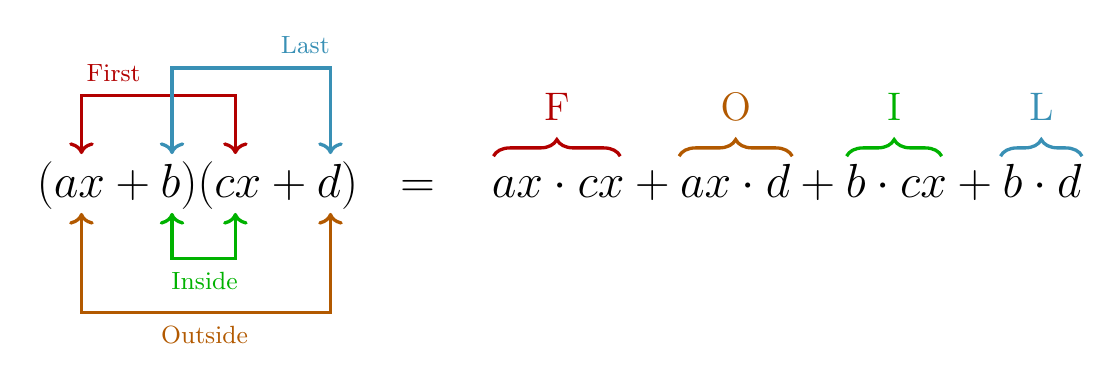
\begin{tikzpicture}[scale=1.15]
 \node[anchor=west] at (0.25,2.0) {\LARGE$(ax+b)(cx+d) \ \ = \quad ax\cdot cx  + ax\cdot d + b \cdot cx  + b\cdot d$};

 \draw[very thick, red!70!black,<->] (0.85,2.35)--(0.85,3.0)--(2.55,3.0)--(2.55,2.35);
   \node[right] at (0.8,3.25) {\color{red!70!black} \small First};
 \draw[very thick, cyan!70!black,<->] (1.85,2.35)--(1.85,3.3)--(3.6,3.3)--(3.6,2.35);
   \node[left] at (3.7,3.55) {\color{cyan!70!black} \small Last};
 \draw[very thick, green!70!black,<->] (1.85,1.7)--(1.85,1.2)--(2.55,1.2)--(2.55,1.7);
   \node[ ] at (2.21,0.95) {\color{green!70!black} \small Inside};
 \draw[very thick, orange!70!black,<->] (0.85,1.7)--(0.85,0.6)--(3.6,0.6)--(3.6,1.7);
   \node[ ] at (2.21,0.35) {\color{orange!70!black} \small Outside};


 %braces
 \draw [very thick,decorate, red!70!black, decoration={brace, amplitude=6pt, raise=2.5pt}] (5.4,2.25)--(6.8,2.25) node [ midway, above=0.4cm] {\Large \color{red!70!black} F};
 \draw [very thick,decorate, orange!70!black, decoration={brace, amplitude=6pt, raise=2.5pt}] (7.45,2.25)--(8.7,2.25) node [ midway, above=0.4cm] {\Large \color{orange!70!black} O};
 \draw [very thick,decorate, green!70!black, decoration={brace, amplitude=6pt, raise=2.5pt}] (9.3,2.25)--(10.35,2.25) node [ midway, above=0.4cm] {\Large \color{green!70!black} I};
 \draw [very thick,decorate, cyan!70!black, decoration={brace, amplitude=6pt, raise=2.5pt}] (11,2.25)--(11.9,2.25) node [ midway, above=0.4cm] {\Large \color{cyan!70!black} L};
 \end{tikzpicture}
\newpage
\subsection{Common Number Sets}

\subsubsection*{Natural Numbers ($\mathbb{N}$)}
The set of natural numbers is denoted by $\mathbb{N}$ and includes all positive integers from 1 onwards. 
\[ \mathbb{N} = \{1, 2, 3, 4, \ldots\} \]

\subsubsection*{Integers ($\mathbb{Z}$)}
The set of integers is denoted by $\mathbb{Z}$. It includes all whole numbers, both positive and negative, including zero.
\[ \mathbb{Z} = \{\ldots, -3, -2, -1, 0, 1, 2, 3, \ldots\} \]

\subsubsection*{Rational Numbers ($\mathbb{Q}$)}
The set of rational numbers is denoted by $\mathbb{Q}$. It includes all numbers that can be expressed as a fraction of two integers, where the denominator is not zero.
\[ \mathbb{Q} = \left\{\frac{a}{b} \mid a,b \in \mathbb{Z}, b \neq 0\right\} \]

\subsubsection*{Real Numbers ($\mathbb{R}$)}
The set of real numbers is denoted by $\mathbb{R}$. It includes all rational and irrational numbers, forming the continuum on the number line.

\subsubsection*{Complex Numbers ($\mathbb{C}$)}
The set of complex numbers is denoted by $\mathbb{C}$. It includes all numbers of the form $a + bi$, where $a$ and $b$ are real numbers and $i$ is the imaginary unit.

\begin{figure}[ht]
    \centering
    \includegraphics[width=0.35\textwidth]{imgs/number-sets-nzqar.jpg}
    \end{figure}

\newpage    
\section{Unit 1}
\subsection{Power Functions}

\begin{minipage}[t]{\textwidth}
Linear and Quadratic functions are the two most encountered polynomial functions. Polynomials are defined as follows...

A polynomial expression is an expression of the form
\[
a_n x^n + a_{n-1} x^{n-1} + a_{n-1} x^{n-2} + \ldots + a_3 x^3 + a_2 x^2 + a_1 x + a_0,
\]
where
\begin{itemize}
    \item \( n \) is a whole number
    \item \( x \) is a variable
    \item the coefficients \( a_0, a_1, \ldots, a_n \) are real numbers
    \item the degree of the function is \( n \), the exponent of the greatest power of \( x \)
    \item \( a_n \), the coefficient of the greatest power of \( x \), is the leading coefficient
    \item \( a_0 \), the term without a variable, is the constant term
\end{itemize}

A polynomial function has the form
\[
f(x) = a_n x^n + a_{n-1} x^{n-1} + a_{n-2} x^{n-2} + \ldots + a_5 x^3 + a_2 x^2 + a_1 x + a_0
\]

Power functions, the simplest polynomial functions, have one term and transform into a general polynomial function when transformed.
\end{minipage}

\vspace{0.5cm}

\begin{center}
\begin{minipage}[t]{0.8\textwidth}
\centering
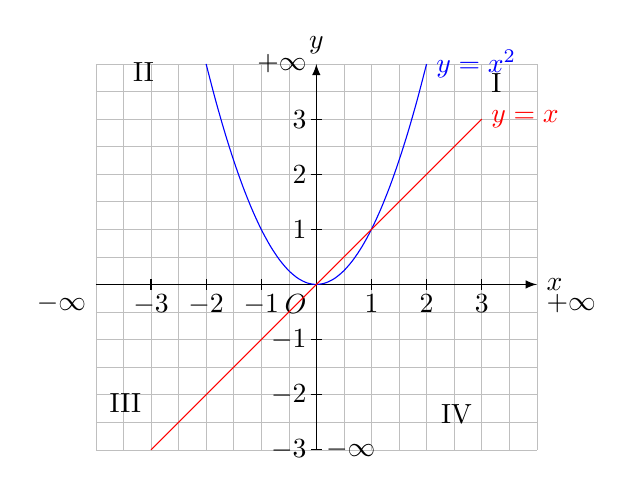
\begin{tikzpicture}[>=latex, scale=0.7]
    % Grid
    \draw[xstep=0.5,ystep=0.5,gray!50,very thin] (-4,-3) grid (4,4);
    % Axes
    \draw[->] (-4,0) -- (4,0) node[right] {$x$};
    \draw[->] (0,-3) -- (0,4) node[above] {$y$};
    % Label x and y axes
    \foreach \x in {-3,-2,-1,1,2,3}
        \draw (\x,-0.1) -- (\x,0.1) node[below=2pt] {$\x$};
    \foreach \y in {-3,-2,-1,1,2,3}
        \draw (-0.1,\y) -- (0.1,\y) node[left=2pt] {$\y$};
    % Label infinity
    \node[below right] at (4,0) {$+\infty$};
    \node[left] at (0,4) {$+\infty$};
    \node[below left] at (-4,0) {$-\infty$};
    \node[right] at (0,-3) {$-\infty$};
    % Label quarters
    \node[below left] at (0,0) {$O$};
    \node[below right] at (3,4) {I};
    \node[above right] at (-3.5,3.5) {II};
    \node[above left] at (-3,-2.5) {III};
    \node[below left] at (3,-2) {IV};
    % Plot y=x^2
    \draw[domain=-2:2,smooth,variable=\x,blue] plot ({\x},{\x*\x}) node[right] {$y=x^2$};
    % Plot y=x
    \draw[domain=-3:3,smooth,variable=\x,red] plot ({\x},{\x}) node[right] {$y=x$};
\end{tikzpicture}
\end{minipage}\\


\end{center}

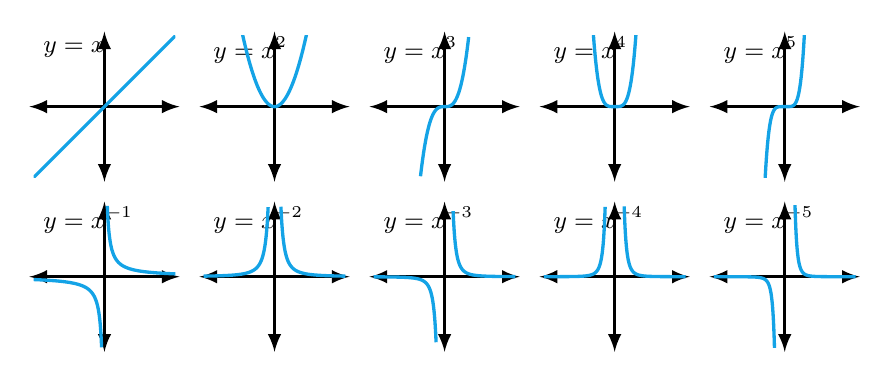
\begin{tikzpicture}[scale=0.3] 

\foreach \e/\d [count=\i] in {1/5,2/2.3,3/1.7,4/1.5,5/1.5,-1/0.2,-2/0.45,-3/0.6,-4/0.67,-5/0.7} {
  \ifnum\e < 0
    \pgfmathsetmacro\row{0};
  \else 
    \pgfmathsetmacro\row{1};
  \fi

  \begin{scope}[scale=0.6, xshift=abs(\e)*12 cm, yshift=\row*12 cm] 
    \ifnum\e = 1
      \node[right] at (-5,4) {\small $y=x$};
    \else 
      \node[right] at (-5,4) {\small $y=x^{\e}$};
    \fi

    \draw[latex-latex, very thick] (-5.3,0)--(5.3,0);
    \draw[latex-latex, very thick] (0,-5.3)--(0,5.3);

    \begin{scope}
      \clip(-5,-5) rectangle (5,5);
      \ifnum\e > 0
        \draw[domain=-\d:\d, smooth, variable=\x, Cerulean, samples=120, very thick] plot ({\x},{(\x)^(\e) });
      \else 
        \draw[domain=-5:-\d, smooth, variable=\x, Cerulean, samples=120, very thick] plot ({\x},{(\x)^(\e) });
        \draw[domain=\d:5, smooth, variable=\x, Cerulean, samples=120, very thick] plot ({\x},{(\x)^(\e) });
      \fi 
    \end{scope}
  \end{scope}
}
 
\end{tikzpicture} \\
To explore Polynomial functions along with their powers, functions, special names, graphs, domains, ranges, and end behaviors as well as leading terms, refer to the \href{run:./Unit\%201\%20-\%20Polynomial\%20Functions/Polynomial.tex}{Polynomial.tex} file or \href{https://math.libretexts.org/Bookshelves/Precalculus/Precalculus_1e_(OpenStax)/03%3A_Polynomial_and_Rational_Functions/3.03%3A_Power_Functions_and_Polynomial_Functions}{Power Functions and Polynomial Functions}.

\section*{Understanding Function Properties}

\subsection*{Even and Odd Degree Functions}

\textbf{Even Degree Functions:} Graphs that curve from quadrant 3 to quadrant 1. The higher the exponent the closer the curve gets to the y-axis.\\
\textbf{Odd Degree Functions:} Graphs that make a U-shape. The higher the exponent the U shape gets closer to the y-axis. 

\begin{center}
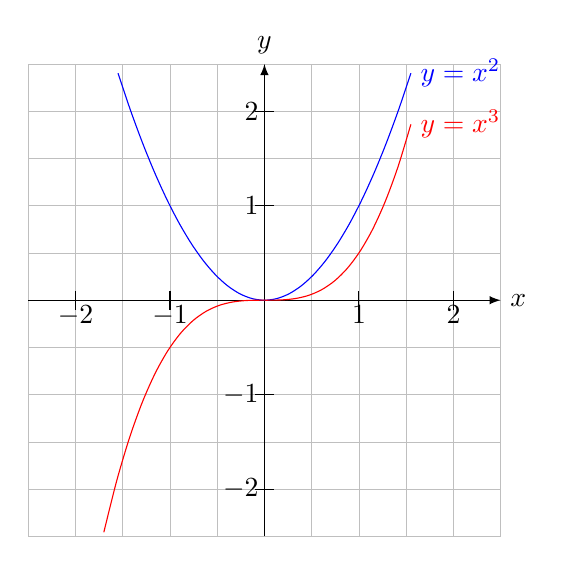
\begin{tikzpicture}[>=latex, scale=1.2]
  % Grid
  \draw[xstep=0.5,ystep=0.5,gray!50,very thin] (-2.5,-2.5) grid (2.5,2.5);
  % Axes
  \draw[->] (-2.5,0) -- (2.5,0) node[right] {$x$};
  \draw[->] (0,-2.5) -- (0,2.5) node[above] {$y$};
  % Labels
  \foreach \x in {-2,-1,1,2}
      \draw (\x,-0.1) -- (\x,0.1) node[below=2pt] {$\x$};
  \foreach \y in {-2,-1,1,2}
      \draw (-0.1,\y) -- (0.1,\y) node[left=2pt] {$\y$};
  % Even function
  \draw[domain=-1.55:1.55,smooth,variable=\x,blue] plot ({\x},{\x*\x}) node[right] {$y=x^2$};
  % Odd function
  \draw[domain=-1.70:1.55,smooth,variable=\x,red] plot ({\x},{0.5*\x*\x*\x}) node[right] {$y=x^3$};
\end{tikzpicture}
\end{center}
\newpage 
\subsection*{Understanding End Behavior}

\textbf{End Behavior:} The end behaviour of a function is the behaviour of the y-values as x increases  (that is, as x approaches positive infinity, $x\to \infty$) and as x decreases (that is, as x approaches negative infinity, $x \to -\infty$)\\

\begin{center}
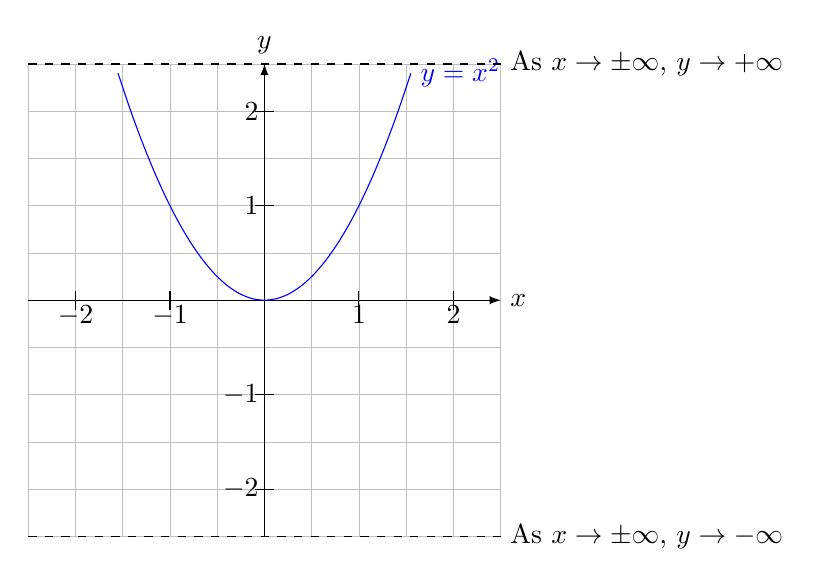
\begin{tikzpicture}[>=latex, scale=1.2]
  % Grid
  \draw[xstep=0.5,ystep=0.5,gray!50,very thin] (-2.5,-2.5) grid (2.5,2.5);
  % Axes
  \draw[->] (-2.5,0) -- (2.5,0) node[right] {$x$};
  \draw[->] (0,-2.5) -- (0,2.5) node[above] {$y$};
  % Labels
  \foreach \x in {-2,-1,1,2}
      \draw (\x,-0.1) -- (\x,0.1) node[below=2pt] {$\x$};
  \foreach \y in {-2,-1,1,2}
      \draw (-0.1,\y) -- (0.1,\y) node[left=2pt] {$\y$};
  % Even function
  \draw[domain=-1.55:1.55,smooth,variable=\x,blue] plot ({\x},{\x*\x}) node[right] {$y=x^2$};
  % End behaviors
  \draw[dashed] (-2.5,2.5) -- (2.5,2.5) node[right] {As $x \rightarrow \pm\infty$, $y \rightarrow +\infty$};
  \draw[dashed] (-2.5,-2.5) -- (2.5,-2.5) node[right] {As $x \rightarrow \pm\infty$, $y \rightarrow -\infty$};
\end{tikzpicture}
\end{center}

\subsection*{Properties of Power Functions}

\textbf{Domain and Range:} 
For power functions, the domain is all real numbers ($x \in \mathbb{R}$), and the range depends on whether the function is even or odd.\\
\textbf{Symmetry:} Power functions exhibit symmetry properties based on whether they are even or odd functions. 

\subsubsection{Deriving Polynomial Functions from Data:}

\begin{table}[h]
    \centering
    \begin{tabular}{|c|c|c|}
    \hline
        \rowcolor[HTML]{EFEFEF}
        $x$ & $y$ & $\Delta f(x)$ \\
        \hline
        1 & 1 & $2-1$\\
        \hline
        2 & 2 & \\
        \hline
        3 & 3 & \\
        \hline
        4 & 4 & $\vdots$ \\
        \hline
        $\vdots$ & $\vdots$ & $\vdots$\\
        \hline
        $m-1$ & $m-1$ & $m-(m-1)$\\
        \hline
        $m$ & $m$ & $m+1-m$\\
        \hline
        $m+1$ & $m+1$ & \\
        \hline
    \end{tabular}
    \caption*{The set of first differences for a linear function remains constant.}
\end{table}

\newpage
\section*{Union and Intersection}
If $A=\{1,3,5,7,9\}$ and $B=\{2,3,5,7$,$\} , what are A \cup B$ and $A \cap B$ ?

We have
$$
\begin{aligned}
& A \cup B=\{1,2,3,5,7,9\} \\
& A \cap B=\{3,5,7\} \cdot 
\end{aligned}
$$


\def\firstcircle{(0,0) circle (1cm)}
\def\secondcircle{(0:1.5cm) circle (1cm)}

\colorlet{circle edge}{blue!50}
\colorlet{circle area}{blue!20}

\tikzset{
    filled/.style = {fill=circle area, draw=circle edge, thick},
    outline/.style = {draw=circle edge, thick},
    F/.style = {draw, inner sep=7mm, fit=(current bounding box),
                node contents={}}
}



\begin{center}
\end{center}

\begin{figure}[h]
    \centering
    \begin{minipage}[t]{0.45\linewidth} 
        \centering   
        \begin{tikzpicture}
            \draw[filled] \firstcircle node {$A$}
                          \secondcircle node {$B$};
            \node (a) [F];                 
            \node[below left] at (a.north east) {$A \cup B$};
        \end{tikzpicture}
        \caption{Presentation of sets union by Venn diagram}
        \label{fig:ven-1a}
    \end{minipage}
    \hfil
    \begin{minipage}[t]{0.45\linewidth}
        \centering
        \begin{tikzpicture}
            \begin{scope}
                \clip \firstcircle;
                \fill[filled] \secondcircle;
            \end{scope}
            \draw[outline] \firstcircle node {$A$};
            \draw[outline] \secondcircle node {$B$};
            \node (a) [F];
            \node[below left] at (a.north east) {$A \cap B$};
        \end{tikzpicture}
        \caption{Presentation of sets intersection by Venn diagram}
        \label{fig:ven-1b}
    \end{minipage}% end of subfloat
\end{figure}


Feel free to learn more in \href{https://brilliant.org/wiki/sets-union-and-intersection-easy/#:~:text=The%20union%20of%202%20sets,the%20symbol%20is%20%E2%88%AAnion.}{Union and intersections}

\subsection{Characteristics of Polynomial Function}

A general note: Terminology of polynomial functions:\\
\begin{figure}[h]
    \centering
    \includegraphics[width=0.6\textwidth]{imgs/polynomial.jpg}
\end{figure}\\
Finite Differences: The nth differences for a polynomial of degree n will all
be the same, and this common difference will be equal to the product of n!
and the leading coefficient $(a_n)$.
\begin{align*}
\text{Common Difference} &= a_nn! (a_n \times n!)\\
&= a_n[n \times (n-1) \times (n-2) \times \cdots \times 3 \times 2 \times 1]
\end{align*}
where, 
\begin{itemize}
    \item \(a_n\) represents the \(n\)th term of the arithmetic sequence.
    \item \(n!\) represents the factorial of \(n\), which is the product of all positive integers up to \(n\). For example, \(5! = 5 \times 4 \times 3 \times 2 \times 1\).
\end{itemize}

\subsubsection*{Example:}The finite differences are taken for a polynomial function, and the 6th differences are found to all be -2880. What was the
leading coefficient of the polynomial function.
Given:
\[
\text{Common Difference} = -2880 = a \times 6!
\]

We are trying to find the value of \(a\). So, let's solve for \(a\):

\[a = \frac{-2880}{6!} = \frac{-2880}{720} = -4\]

So, the value of \(a\) is indeed \(-4\).
\subsubsection{Anatomy of a Polynomial Function:}
\begin{figure}[ht]
    \centering
    \includegraphics[width=0.6\textwidth]{imgs/anatomyofapolynomialfunction.png}
\end{figure}


To learn more about the characteristics of polynomial functions, you can visit the following link: \href{https://mathematicalmysteries.org/characteristics-of-polynomials/}{Characteristics of Polynomial Function}.

\subsubsection{Local Minimum and Maximum Points}
Let's look at the graph of the polynomial function defined by $x^3+x^2$.

\begin{minipage}{0.6\linewidth}
\centering
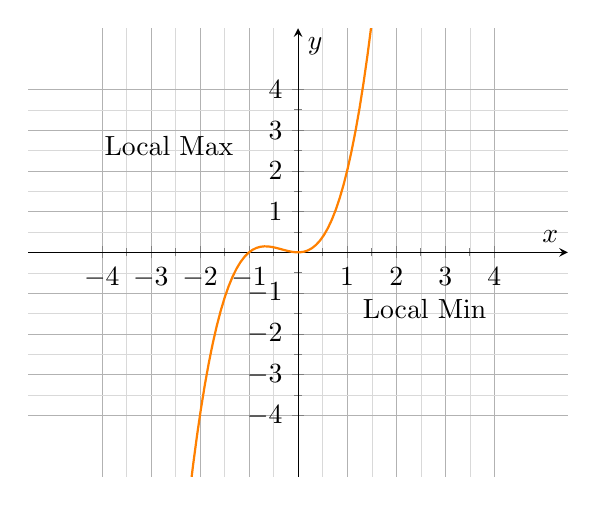
\begin{tikzpicture}
\begin{axis}[
    xlabel=$x$,
    ylabel=$y$,
    axis lines=middle,
    xmin=-5,
    xmax=5,
    ymin=-5,
    ymax=5,
    xtick={-4,...,4},
    ytick={-4,...,4},
    grid=both,
    grid style={line width=.1pt, draw=gray!30},
    major grid style={line width=.2pt,draw=gray!60},
    minor tick num=1,
    enlargelimits={abs=0.5},
]
% Plot the function
\addplot[domain=-4:4, samples=100, thick, orange] {x^3 + x^2};

% Local minimum and maximum points
\node[circle, inner sep=2pt,label={above right: Local Min}] at (axis cs:1,-2) {};
\node[circle,inner sep=2pt,label={above left:Local Max}] at (axis cs:-1,2) {};
\end{axis}
\end{tikzpicture}
\end{minipage}%
\begin{minipage}{0.4\linewidth}
Looks more $f(x)=x^3$ than $f(x)=x^2$, but there is a small change we now have "bumps" on the graph.
\end{minipage}
In general, polynomial function graphs consist of a smooth curve with a series of hills and valleys. The hills and valleys are called turning points. Each \textbf{turning point} corresponds to a \textbf{local maximum} or \textbf{local minimum point}. 
\newpage 
\textbf{Finite Differences:}{ (used to find leading terms and determine degree from a table of values)}
\subsubsection*{Example 1:} 
Recall for linear functions $f(x) = 3x + 2$ we could make a table of values 

\[
\begin{array}{|c|c|c|}
\hline
x & f(x) & \text{First Difference} \\
\hline
0 & 2 & \\
1 & 5 & 3 \\
2 & 8 & 3 \\
3 & 11 & 3 \\
4 & 14 & 3 \\
5 & 17 & 3 \\
\hline
\end{array}
\]
First Difference is constant, so degree is equal to 1 and leading coefficient is 3 
\subsubsection*{Example 2:}

\[
\begin{array}{|c|c|c|c|}
\hline
x & y & \text{1st Difference} & \text{2nd Difference} \\
\hline
0 & 1 & & \\
1 & 6 & 5 & \\
2 & 17 & 11 & 6 \\
3 & 34 & 17 & 6 \\
4 & 57 & 23 & 6 \\
5 & 86 & 29 & 6 \\
\hline
\end{array}
\]
Second Difference is constant, so degree is equal to 2 but the leading coefficient is not 6 it should be 3. So how do we account for this?
For a polynomial of degree \( n \), where \( n \) is a positive integer, the \( n \)th differences:
\begin{itemize}
    \item are constant (equal)
    \item have the same sign as the leading coefficient
    \item are equal to \( a(n!) \), where \( a \) is the leading coefficient
\end{itemize}

Factorial (!) means: \( n! = n(n - 1)(n - 2)(n - 3) \dotsm (2)(1) \)

For example, \( 5! = 5 \times 4 \times 3 \times 2 \times 1 = 120 \).

So for our example above, the second difference is constant, so the degree is equal to 2, but the leading coefficient is \( a(n!) \):

\[ 6 = a(2!) \text{ because } n = 2 \]
\[ 6 = a(2)(1) \]
\[ 6 = 2a \]
\[ 3 = a \]

\subsubsection{Key Features of Polynomial Functions with Odd Degree}

\subsubsection*{Description}

\begin{itemize}
    \item Odd-degree polynomials have at least one zero, up to a maximum of \( n \) x-intercepts, where \( n \) is the degree of the function.
    \item The domain is \( x \in \mathbb{R} \) and the range is \( y \in \mathbb{R} \).
    \item They have no absolute maximum point and no absolute minimum point.
    \item They may have point symmetry.
\end{itemize}

\subsubsection*{Graphical Representation}

\begin{center}
\begin{tikzpicture}[scale=0.7]
% Axes
\draw[-{Stealth}] (-5,0) -- (5,0) node[below] {\( x \)};
\draw[-{Stealth}] (0,-5) -- (0,5) node[left] {\( y \)};
% Function
\draw[domain=-1:1,smooth,variable=\x,red] plot ({\x},{\x^3-\x});
% Annotations
\draw[dashed] (1,0) node[below] {\( 1 \)} -- (1,0 |- 0,1) node[left] {\( f(1) \)};
\draw[dashed] (-1,0) node[below] {\( -1 \)} -- (-1,0 |- 0,-1) node[right] {\( f(-1) \)};
\end{tikzpicture}
\end{center}

\subsubsection*{Positive Leading Coefficient}

\begin{itemize}
    \item Graph extends from quadrant 3 to quadrant 1.
    \item Alternatively, as \( x \to -\infty \), \( y \to -\infty \) and as \( x \to \infty \), \( y \to \infty \).
\end{itemize}

\subsubsection*{Negative Leading Coefficient}

\begin{itemize}
    \item Graph extends from quadrant 2 to quadrant 4.
    \item Alternatively, as \( x \to -\infty \), \( y \to \infty \) and as \( x \to \infty \), \( y \to -\infty \).
\end{itemize}




\subsubsection{Key Features of Polynomial Functions with Even Degree}

\subsubsection*{Description}

\begin{itemize}
    \item Even-degree polynomials may have no zeros, up to a maximum of \( n \) x-intercepts, where \( n \) is the degree of the function.
    \item The domain is \( \{x \in \mathbb{R}\} \).
    \item They may have line symmetry.
\end{itemize}

\subsubsection*{Graphical Representation}

\begin{center}
\begin{tikzpicture}[scale=0.44]
% Axes
\draw[-{Stealth}] (-5,0) -- (5,0) node[below] {\( x \)};
\draw[-{Stealth}] (0,-5) -- (0,5) node[left] {\( y \)};
% Function
\draw[domain=-2:2,smooth,variable=\x,blue] plot ({\x},{\x^2-2});
% Annotations
\draw[dashed] (1,0) node[below] {\( 1 \)} -- (1,0 |- 0,1) node[left] {\( f(1) \)};
\draw[dashed] (-1,0) node[below] {\( -1 \)} -- (-1,0 |- 0,1) node[left] {\( f(-1) \)};
\end{tikzpicture}
\end{center}

\subsubsection*{Positive Leading Coefficient}

\begin{itemize}
    \item Graph extends from quadrant 2 to quadrant 1.
    \item Alternatively, as \( x \to -\infty \), \( y \to \infty \) and as \( x \to \infty \), \( y \to \infty \).
    \item The range is \( \{y \in \mathbb{R} | y \geq a\} \), where \( a \) is the absolute minimum value of the function.
    \item It will have at least one minimum point.
    \item It will have an absolute minimum point.
\end{itemize}

\subsubsection*{Negative Leading Coefficient}

\begin{itemize}
    \item Graph extends from quadrant 3 to quadrant 4.
    \item Alternatively, as \( x \to -\infty \), \( y \to -\infty \) and as \( x \to \infty \), \( y \to -\infty \).
    \item The range is \( \{y \in \mathbb{R} | y \leq a\} \), where \( a \) is the absolute maximum value of the function.
    \item It will have at least one maximum point.
    \item It will have an absolute maximum point.
\end{itemize}


\subsection{Graphs of Polynomial Functions}
\begin{itemize}
    \item The function must be in \textcolor{red}{factored} form to find the x-intercepts.
    \item Plot the x-intercepts, and the y-intercept(get h y-intercept by subbing \textcolor{red}{0} in for x)
    \item Use an \textcolor{red}{interval} test to determine the sign of the polynomial in the intervals divided by the x-intercepts.
    \item The function $f(x)=(x-3)(x-1)(x+2)^2(x+5)^3$ is of degree 7. It has \textcolor{red}{4} intercepts. The zero from the factor $(x+2)^2$ is repeated and so is said to have \textcolor{red}{order} of 2. The zero from the factor $(x+5)^3$ is repeated and so is said to have order $3$.
    \item The function will pass through the axis at any zero with an \textcolor{red}{odd} order, and just skim the x-axis for zeros with an \textcolor{red}{even} order.
    \item For a zero of order 1, the function will pass through the x-axis looking \textcolor{red}{linear}.
    \item For a zero of order 2 the function will pass through the ax-s looking \textcolor{red}{quadratic} $\dots$ and so on $\dots$
\end{itemize}

\begin{figure}[h]
    \centering
    \includegraphics[width=0.75\textwidth]{imgs/image001.png}
    \end{figure}


\subsection{Symmetry in Polynomial Functions}
A polynomial function is called an even function if the exponent of each term of the equation is even. The value of the function would be the same if you subbed in a positive value or its opposite negative value.
$$f(x) = f(-x)$$ Because of this, the function will be symmetric about the y-axis

A polynomial function is called an odd function if the exponent of each term of the equation is odd. The value of the function would have the opposite sign if you
subbed in a positive value of its opposite negative value
$$f(-x) = -f(x)$$
Because of this, the function will be symmetric about the origin. 
\subsection{Transformations of Power Functions}
\begin{itemize}
    \item \textbf{Vertical Shift:} Value of $C$ in $f(x) = a[k(x - d)]^n + c$
    \begin{itemize}
        \item $C > 0$: Shift $C$ units up
        \item $C < 0$: Shift $C$ units down
    \end{itemize}
    
    \item \textbf{Horizontal Shift:} Value of $h$ in $f(x) = a[k(x - d)]^n + c$
    \begin{itemize}
        \item $d > 0$: Shift $|d|$ units right
        \item $d < 0$: Shift $|d|$ units left
    \end{itemize}
    
    \item \textbf{Vertical Stretch/Compression and Reflection:} Value of $a$ in $f(x) = a[k(x - d)]^n + c$
    \begin{itemize}
        \item $a > 1$ or $a < -1$: Vertical stretch by a factor of $|a|$
        \item $-1 < a < 1$: Vertical compression by a factor of $|a|$
        \item $a < 0$: Vertical reflection (reflection in the $x$-axis)
    \end{itemize}
    
    \item \textbf{Horizontal Compression/Stretch and Reflection:} Value of $k$ in $f(x) = a[k(x - d)]^n + c$
    \begin{itemize}
        \item $k > 1$ or $k < -1$: Horizontal compression by a factor of $|k|$
        \item $-1 < k < 1$: Horizontal stretch by a factor of $|k|$
        \item $k < 0$: Horizontal reflection (reflection in the $y$-axis)
    \end{itemize}
\end{itemize}

\textbf{Note:}
\begin{itemize}
    \item $C$ and $d$ cause vertical transformations and therefore affect the $y$-coordinates of the function.
    \item $a$ and $k$ cause horizontal transformations and therefore affect the $x$-coordinates of the function.
    \item When applying transformations to a parent function, make sure to apply the transformations represented by $C$ and $d$ before the transformations represented by $a$ and $k$.
    \item We can use the mapping $(x,y) \to \left( \frac{x}{k}+d, ay+c\right)$ to transform every point on the original power function into the new power function
\end{itemize}
\newpage
\subsection*{Intro To Absolute Value}
\textbf{Absolute value:} $f(x)= |x|$, the definition that "x" is from the origin on the number line. \\ 
In general:\\
$$
|f(x)|=
\begin{cases}
f(x) &, f(x) \ge 0\\
-f(x) &, f(x) < 0
\end{cases}
$$
The absolute value of a number is its distance from 0. For example, the absolute value of 4 is 4:
\begin{center}
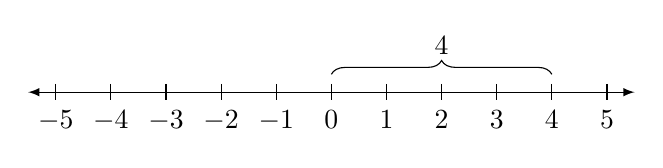
\begin{tikzpicture}[>=latex, scale=0.7]
    \draw[latex-latex] (-5.5,0) -- (5.5,0);
    \foreach \x in {-5,...,5}
    \draw (\x,0.15) -- (\x,-0.15) node[below] {$\x$};
   
    \draw[-,decorate,decoration={brace,amplitude=5pt,raise=1.5ex}]
      (0,0) -- (4,0) node[midway,above=1em]{$4$};
\end{tikzpicture}
\end{center}

This seems kind of obvious. Of course, the distance from 0 to 4 is 4. Where absolute value gets interesting is with negative numbers. \\ \\
For example, the absolute value of -4 is also 4:
\begin{center}
    
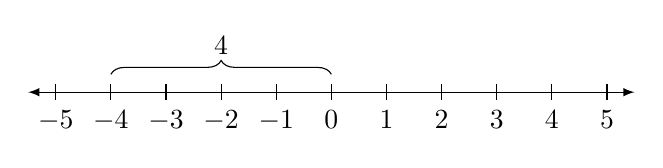
\begin{tikzpicture}[>=latex, scale=0.7]
    % Axis
    \draw[latex-latex] (-5.5,0) -- (5.5,0);
    \foreach \x in {-5,...,5}
    \draw (\x,0.15) -- (\x,-0.15) node[below] {$\x$};
   
    % Brace
    \draw[-,decorate,decoration={brace,amplitude=5pt,raise=1.5ex}]
      (-4,0) -- (0,0) node[midway,above=1em]{$4$};
\end{tikzpicture}
\end{center}

\subsection*{The absolute value symbol}
The symbol for absolute value is a bar \texttt{|} on each side of the number. \\
For example, instead of writing
"the absolute value of -6", we can just write |-6|. \\\\
\textbf{Odd functions:} A function $f(x)$ is odd if $f(-x)= -f(x)$. Symmetric about the origin or reflection along both the x and y axis. \\ 
$\quad f(x)=-2x^3+x$, is an odd function since $f(-x)=-2(-x)^3+(-x)$ \\  \\
\textbf{Note:}$$f(-x)=-f(x)$$ \\ 
For polynomial functions, the function is an odd function if all exponents are odd. \\ 
\textbf{Even functions:} A function $f(x)$ is even if $f(-x)=f(x)$. Symmetric about the y-axis. \\ 
i.e $\quad f(x)=3x^4+2x^2-2$, is an even function since function if all the exponents are even. \\ 
\newpage 
\subsection{Slopes of Secants and Average Rate of Change}
\textbf{Key Concepts}

\begin{itemize}
    \item A secant is a straight line that connects two points on a curve.
    \item Rate of Change (Slope) is a measure of how quickly one quantity (the dependent variable) changes with respect to another quantity (the independent variable).
There are two types of rates of change, average and instantaneous.
\end{itemize}



\subsubsection{Average rates of change}
    represent the rate of change over a specified interval corresponding to the slope of a secant between two points $P_1 (x_1, y_1)$ and $P_2(X_2,Y_2)$ on a curve
\begin{figure}[h]
    \centering
    \includegraphics[width=0.9\textwidth]{imgs/Slopes of Secants and Average Rate of Change.png}
    \end{figure}
    
An average rate of change can be determined by calculating the slope between two points given in a table of values or by using an equation.

\subsection{Slopes of Tangents and Instantaneous Rate of Change}
\begin{enumerate}
    \item A tangent to a curve is a line that intersects a curve at exactly one point.
    \item An instantaneous rate of change corresponds to the slope of a tangent at a point on a curve.
    \item An approximate value for an instantaneous rate of change at a point may be determined using....
\end{enumerate}
\begin{itemize}
\item a graph, either by estimating the slope of a secant passing through that point OR by sketching the tangent and estimating the slope between the tangent point and a second point on the approximate tangent line.
\item a table of values, by estimating the slope between the point and a nearby point in the table.
\item an equation, by estimating the slope using a very short interval between the tangent point and a second point found using the equation.
\end{itemize}
\subsubsection{Relationship Between the Slope of Secants and the Slope of a Tangent}
\begin{itemize}
    \item As a point Q becomes very close to a tangent point P, the slope of the secant line becomes closer to (approaches) the slope of the tangent line.
    \item Often an arrow is used to denote the word "approaches". So, the above statement may be written as follows:
    \item As Q$\to$ P, the slope of the secant PQ the slope of the tangent at P.
    \item Thus, the average rate of change between P and Q becomes closer to the value of the instantaneous rate of change at P.
\end{itemize}
\begin{figure}[h]
    \centering
    \includegraphics[width=1\textwidth]{imgs/l5olF.png}
    \end{figure}

  When $x=0, f(0)=0$, and when $x=3, f(3)=9$. The slope of the secant from $(0,0)$ to $(3,9)$ is
$$
\begin{aligned}
\frac{\Delta f(x)}{\Delta x} & =\frac{9-0}{3-0} \\
& =3
\end{aligned}
$$

When $x=1, f(1)=1$. The slope from $(1,1)$ to $(3,9)$ is
$$
\begin{aligned}
\frac{\Delta f(x)}{\Delta x} & =\frac{9-1}{3-1} \\
& =4
\end{aligned}
$$

When $x=2, f(2)=4$. The slope from $(2,4)$ to $(3,9)$ is
$$
\begin{aligned}
\frac{\Delta f(x)}{\Delta x} & =\frac{9-4}{3-2} \\
& =5
\end{aligned}
$$  


\section{Unit 2}

\subsection{The Remainder Theorem - Part 1}
\textbf{Long Division:}
Check if you remember how to do long division with constants...
\[
\begin{array}{c|ccccc}
4156 \text{r} 5 & 6 & 2 & 3 & 4 & 5 \\
\multicolumn{1}{r}{15} & 6 & 0 & \downarrow & \Big\downarrow & \bigg\downarrow \\
\cline{2-4}
 &  & 2 & 3 &  \\
 & & 1 & 5 &  \\
\cline{2-4}
 &  &  & 8 & 4 \\
 &  & & 7 & 5\\
\cline{4-6}
 &  &  &  & 9 & 5 \\
 &  &  &  & 9 & 0 \\
\cline{5-6}
 &  &  &  & & 5 \\
\end{array}
\]



The process of long division is similar with polynomials.
\subsubsection*{Example 1: Divide $3x^4-12x^3-20x^2-30x+2$ by $x-5$}

$$\polylongdiv{3x^4-12x^3-20x^2-30x+2}{x-5}$$
You know you are finished when the degree of the remainder is less than the
degree of the divisor. For example – we have a linear divisor so our remainder
will be constant. \\ \\ 
If we state our result in quotient form it would look like this…
$$\frac{3x^4-12x^3-20x^2-30x+2}{x-5}=3x^3+3x^2-5x-55-\frac{273}{(x-5)}$$
In general that would be...
$$\frac{P(x)}{(x-b)}=Q(x)+\frac{R}{(x-b)}$$
\newpage
Often I’ll want you to conclude a division question with a division statement
in the proper form.\\\\
\begin{center}
Original Polynomial = Divisor x Quotient + Remainder.
\end{center}
In function notation we write:
$$P(x)=(x-b)Q(x)+\mathbb{R}$$
For the example above, the division statement will be
\begin{figure}[h]
    \centering
    \includegraphics[width=0.6\textwidth]{imgs/division statement.png}
\end{figure}\\
Note: if you expand the right side of the division statement and simplify, you
should get what’s on the left side.

\subsubsection*{Example 2: Divide $6z^3+13z^2-9$ by $2z+3$}
You must always place the polynomial in descending powers of the variable. If
one power of the variable is missing, it means its coefficient was zero, and you
need to put it in as a placeholder.


\begin{gather*}
\parbox{0.4\linewidth}{
    \polylongdiv{6x^3 + 13x^2 + 0x - 9}{2x + 3}
}
\end{gather*}
Since the remainder is zero, we know that the divisor went evenly into the
polynomial. That makes it a factor of the original polynomial.
\newpage 
\subsection*{Synthetic Division}
Synthetic Division – used when you have a linear divisor
To use synthetic division you must have
\begin{itemize}
    \item a linear divisor where the coefficient of the variable is ONE.
    \item a polynomial written in descending powers of the variable.
    \item if you are missing a power of the variable, you must fill in a zero for its coefficient.
\end{itemize}

Now, we only write the coefficients and fill in the variable when we are finished.
\subsubsection*{Example 1: Divide $5w^2-4w-2+w^3$ by w-1}
\begin{figure}[h]
    \centering
    \includegraphics[width=0.6\textwidth]{imgs/synthetic division.png}
\end{figure}


The final numbers $(1,6,2,0)$ represent the coefficients of the quotient, starting with the power that is one less than the original polynomial. In this case, our answer will be $w^2 + 6w + 2$, and the last number is the remainder (zero).\\

So our division statement is: $P(x)=(w-1)(1w^2+6w+2)$
\subsubsection*{Example 2: Divide $6w^4-3x^3+2x-5$ by w+3 }
$$\polyhornerscheme[x=-3]{6x^4-3x^3+2x-5}$$
\newpage 
\subsection{The Remainder Theorem - Part 2}
\subsubsection*{Example 1.} Divide the polynomial $P(x)=x^3-2x^2-4$ by $x-2$.\\
We’ll use synthetic division…
$$\polyhornerscheme[x=2]{x^3-2x^2-4}$$
What I want you to notice is that if evaluate $P(2)$ (remember is the value that makes the bracket zero), this is what I get \\
The final answer is the same as the remainder when we divided. Coincidence? Well, generally if I'm bothering to point out, it is not a coincidence.

\begin{tcolorbox}[enhanced,attach boxed title to top center={yshift=-3mm,yshifttext=-1mm},
  colback=antiquefuchsia!5!white,colframe=antiquefuchsia!75!black,colbacktitle=purple!80!black,
  title=The Remainder Theorm,fonttitle=\bfseries,
  boxed title style={size=small,colframe=red!50!black} ]
 if $P(x)$ is divided by (x-b) and the remainder is constant, then the remainder will be $P(b)$.
\end{tcolorbox}
\begin{align*}
    \textit{Proof:} \quad & \text{P(x) is a polynomial}\\
    &(x-b) \quad \text{is the divisor }\\
    &Q(x) \quad \text{is the quotient }\\
    & R \quad \text{is the remainder }\\
\end{align*}
Then the division statement is
$$
P(x)=(x-b)(Q(x))+R
$$
Evaluate $P(b)$
$$
\begin{aligned}
P(b) & =(b-b)(Q(x))+R \\
& =\underbrace{\cancel{O(Q(x))}}+R_{} \\ 
& =R
\end{aligned}
$$
\begin{tcolorbox}[enhanced,frame style image=blueshade.png,
  opacityback=0.75,opacitybacktitle=0.25,
  colback=blue!5!white,colframe=blue!75!black,
  title=The General Remainder Theorem]
 If $P(x)$ is divided by (ax-b) and the remainder is constant, then the remainder will be $P\left(\frac{b}{a}\right)$ where a, b $\in$ I and a $\neq$ 0
\end{tcolorbox}
\subsubsection*{Example 2: Find the remainder for each division.}
\begin{enumerate}
    \item[a)] $\left( 2x^2-3x+7\right)\div (x+4)$ \\
    \begin{align*}
    P(-4)&=2(-4)^2-3(-4)+7\\
    &=51\\
    &\boxed{R= 51}
    \end{align*}
    \item[b)] $\left( 4x^3-2x^2+6x-1\right) \div (2x-1)$ \\
    \begin{align*}
        P\left(\frac{1}{2}\right)&=4\left(\frac{1}{2}\right)^3-2\left(\frac{1}{2}\right)^2+6\left(\frac{1}{2}\right)-1\\
        &= 2\\
        &\boxed{R=2}
    \end{align*}
\end{enumerate}

\subsubsection*{Example 3.} When the polynomial x3 - 3x2 + kx - 7 is divided by (x-4) the
remainder is 29. What is the value of k?\\
Always start by filling in what you know...

\[ 4^3 - 3(4)^2 + k(4) - 7 = 29 \]

Solving for \( k \):

\[ 64 - 48 + 4k - 7 = 29 \]
\[ 4k + 9 = 29 \]
\[ 4k = 20 \]
\[ k = 5 \]

Therefore, the value of \( k \) is 5.

\newpage
\subsubsection*{Example 4.} For what value of b will the polynomial P(x) = -2x3 + bx2 - 5x + 2\\
have the same remainder when divided by (x - 2) and (x + 1)
If the remainders are the same, we know that P(2) = P(-1) so we sub in and
set them equal.
Given that \( P(2) = P(-1) \), we'll substitute \( x = 2 \) and \( x = -1 \) into the polynomial and set the two expressions equal to each other: \\

For \( x = 2 \):
\[ P(2) = -2(2)^3 + b(2)^2 - 5(2) + 2 \]
\[ P(2) = -16 + 4b - 10 + 2 \]
\[ P(2) = 4b - 24 \]

For \( x = -1 \):
\[ P(-1) = -2(-1)^3 + b(-1)^2 - 5(-1) + 2 \]
\[ P(-1) = 2 + b + 5 + 2 \]
\[ P(-1) = b + 9 \]

Setting \( P(2) \) equal to \( P(-1) \):
\[ 4b - 24 = b + 9 \]
\[ 4b - b = 9 + 24 \]
\[ 3b = 33 \]
\[ b = 11 \]

Therefore, the value of \( b \) is 11.\\\\
\subsection{The Factor Theorem - Part 1}
\begin{tcolorbox}[colback=blue!5!white,colframe=blue!75!black,title=The Factor Theorem ]
    $(x-b)$ is a factor of $P(x)$ if and only $P(b)=0$\\
    $(ax-b)$ is a factor of $P(x)$ if and only if $P\left(\frac{b}{a}\right)$
\end{tcolorbox}

\textit{Proof:} Given $(x-b)$ is a factor of $P(x)$ then\\
That means that the quotient $\frac{P(x)}{(x-b)}$ will have a remainder of zero.


\subsubsection*{Example 1: Is $(x-2)$ a factor of the following polynomials?} 
\begin{enumerate}
    \item[a)] $x^3-7x^2+9x+2$ 
    \begin{align*}
        &=(2)^3-7(2)^2+9(2)+2\\
        &=8-28+18+2\\
        &=0\\
        &\therefore \text{$(x-2)$ is a factor}
    \end{align*}
    \item[b)] $x^3-3x^2+2x-5$
    \begin{align*}
        &=(2)^3-3(2)^2+2(2)-5\\
        &=8-12+4-5\\
        &=-5\\
        &\therefore \text{$(x-2)$ is NOT a factor}
    \end{align*}
\end{enumerate}

\subsection*{Integral Zero Theorem}

Given the polynomial in factored form:

\[ P(x) = (2x - 3)(x + 4)(x - 5) \]

To find the constant term in the expanded polynomial, we multiply all the constant terms of the factors, which are \( -3 \), \( 4 \), and \( -5 \). Thus, the constant term should be:

\[ (-3) \times 4 \times (-5) = 60 \]

So, if this polynomial were in expanded form, we would know that any zeros would have to be a factor of \textcolor{blue}{60}. \\

In general:
\begin{tcolorbox}[colback=red!5!white,colframe=red!75!black]
For $(x-b)$  to be a factor of the polynomial $P(x)$, b must be
a factor of the constant term of $P(x)$.
\end{tcolorbox}

\subsubsection*{Example 2. Factor the following...}
$$x^3 + 2x^2 -5x - 6$$
We need to divide out a linear factor, then we can employ our
methods of factoring quadratics. \\
By the integral zero theorem, any zeros we find (that are integers)
will be factors of 6. \\
When you check, always start with $\pm 1$.\\\\
Feel free to look more explanation on \href{https://www.youtube.com/watch?v=7Hny2n6t83Y}{MHF4U U2L3 The Factor Theorem Part 1} at 6:08.

\subsection*{The Rational Zero Theorem}
The Rational Zero Theorem provides a useful tool for identifying potential rational roots of a polynomial equation. It states that if a polynomial function

\[ P(x) = a_nx^n + a_{n-1}x^{n-1} + \ldots + a_1x + a_0 \]

where \( a_n, a_{n-1}, \ldots, a_1, a_0 \) are integers with \( a_n \neq 0 \), has any rational roots, then these roots must be of the form \( \pm \frac{p}{q} \), where \( p \) is a factor of the constant term \( a_0 \) and \( q \) is a factor of the leading coefficient \( a_n \).

In simpler terms, if a polynomial has rational roots, they can be expressed as \( \pm \frac{p}{q} \), where \( p \) divides evenly into the constant term and \( q \) divides evenly into the leading coefficient.

This theorem offers a systematic approach to identifying potential rational roots, which can significantly streamline the process of finding all roots of a polynomial equation.

\subsection{Sum and Difference of Cubes}

The formulas for factoring sums and differences of cubes are as follows:

\subsubsection*{Sum of Cubes:}

\[ a^3 + b^3 = (a + b)(a^2 - ab + b^2) \]

\subsubsection*{Difference of Cubes:}

\[ a^3 - b^3 = (a - b)(a^2 + ab + b^2) \]

These formulas can be derived by expanding the corresponding expressions.

\subsubsection*{Examples}

\begin{enumerate}
    
    \item[a)] \textbf{Sum of Cubes (Numeric Example):} Factor \( 8a^3 + 27b^3 \).
    \[ 8a^3 + 27b^3 = (2a)^3 + (3b)^3 \]
    \[ = (2a + 3b)(4a^2 - 6ab + 9b^2) \]
    
    \item[b)] \textbf{Difference of Cubes (Numeric Example):} Factor \( 64x^3 - 27y^3 \).
    \[ 64x^3 - 27y^3 = (4x)^3 - (3y)^3 \]
    \[ = (4x - 3y)(16x^2 + 12xy + 9y^2) \]
\end{enumerate}

These formulas provide a convenient way to factor expressions involving cubes, which can be useful in various algebraic manipulations.
\newpage 
\subsection{Solving Polynomial Equations}
\begin{itemize}
    \item A polynomial inequality results when the equal sign in a polynomial equation is replaced
with an inequality symbol. < >
    \item The real zeros of a polynomial function, or x-intercepts of the corresponding graph, divide
the x-axis into intervals that can be used to solve a polynomial inequality.
    \item Polynomial inequalities may be solved graphically by determining the x-intercepts and
then using the graph to determine the intervals that satisfy the inequality.
    \item A CAS (computer algebra system) on a graphing calculator may be used to solve a polynomial inequality numerically by determining the roots of the polynomial equation and then testing values in each interval to see if they make the inequality true.
\end{itemize}

\begin{minipage}{0.6\textwidth}
Examine the graph of $f(x)=x^2+4x-12$.\\
The x-intercepts are $-6$ and $2$. These correspond to the zeros of the function $f(x)=x^2+4x-12$. By moving from left to right along the x-axis, we can make the following observations.
\begin{itemize}
    \item The function is positive when $x < -6$ since the $y$-values are positive.
    \item The function is negative when $-6 < x < 2$ since the $y$-values are negative.
    \item The function is positive when $x > 2$ since the $y$-values are positive.
\end{itemize}
\end{minipage}%
\vspace{1em}
\begin{minipage}{0.4\textwidth}
\centering
\includegraphics[width=\textwidth]{imgs/graph x^2+4x-12.png}
\end{minipage}

The zeros -6 and 2 divide the x-axis into three intervals: $x < -6, -6 < x < 2$ and $x > 2$. In each interval, the function is either positive or negative. The information can be summarized in a table,
as shown below.     

\begin{table}[ht]
\centering
\begin{tabular}{|c|c|c|c|}
\hline
\textbf{Interval} & $x < -6$ & $-6 < x < 2$ & $x > 2$ \\
\hline
\textbf{Sign of Function} & + & $\bullet$ & + \\
\hline
\end{tabular}
\end{table}

\newpage 
\subsection{Solve Factorable Polynomial Inequalities Algebraically}
\subsubsection{Solving Linear Inequalities}
\begin{itemize}
    \item Solve as you would a regular equation.
    \item Remember to flip the inequality sign when dividing/multiplying by a negative number. 
\end{itemize}
\subsubsection{Solve Polynomial Inequalities}
\begin{itemize}
    \item Factorable inequalities can be solved algebraically by factoring the polynomial, if
necessary, and determining the zeros/roots of the function.
Then...
\begin{enumerate}
    \item Consider all cases, OR
    \item Use intervals and then test values in each interval
\end{enumerate}
    \item Tables and number lines can help organize intervals to provide a visual clue to solutions. 
\end{itemize}

\subsubsection*{Example:} 
Solve the inequality using cases and intervals $(x+3)(2x-3)$
Roots x = - 3, 3/2.\\ 
The polynomial is already in factored form so we have saved a little work. This will not always be true.

We will start with the pure Algebra based solution.
\begin{itemize}
    \item[-] Step 1 - determine the number of possible cases for the inequalities
We have two brackets being multiplied with the goal being to determine when this function will be greater than zero. i.e when is the function positive
The product will be positive when both brackets have a positive value (case 1) or when both brackets have negative values (case 2).
So we have two cases
\item[-] Step 2 - Solve for both cases (determine when are both true)
Case 1
$$
\begin{array}{ll}
x+3>0 & 2 x-3>0 \\
x>-3 & 2 x>3 \\
& x>3 / 2
\end{array}
$$

Both will be positive for numbers less than -3
Case 2
$$
\begin{array}{lll}
\mathrm{x}+3<0 & 2 \mathrm{x}-3<0 \\
\mathrm{x}<-3 & 2 \mathrm{x} & <3 \\
& \mathrm{x} & <3 / 2
\end{array}
$$

Both will be negative for numbers greater than $3 / 2$
\item[-] Step 3 Write your concluding inequality statement
$$
\therefore(x+3)(2 x-3)>0 \text { when } \mathrm{x}<-3 \& \mathrm{x}>3 / 2
$$
\end{itemize}
\newpage 
Let's try this problem a second way using the interval method.\\
\textbf{Intervals:} Start with the idea that this function has the \underline{potential} to change from positive to negative values at the roots. We say potential because it could just touch the axis and bend back.\\
\begin{itemize}
    \item [-] We will create a table to discuss all regions for the function in space,
\item[-] We will test values in these regions in each of the factors to determine the sign of the function.
\item[-] We know the roots of this function are at $\mathrm{x}=-3,3 / 2$ so let us discuss the interval before -3 , between -3 and $3 / 2$, and after $3 / 2$.
\item[-] We will still use the logic from the algebra solution, that both factors must either be positive or negative to provide a result that is $>0$.
\end{itemize}
\begin{tabular}{|c|c|c|c|}
\hline Interval & $x<-3$ & $-3<x<3 / 2$ & $x>3 / 2$ \\
\hline Factors & Try -4 & Try 1 & Try 4 \\
\hline$(x+3)$ & \begin{tabular}{c}
$(-4+3)=-1$ \\
Sign $(-)$
\end{tabular} & \begin{tabular}{c}
$(1+3)=4$ \\
$\operatorname{Sign}(+)$
\end{tabular} & \begin{tabular}{c}
$(4+3)=7$ \\
$\operatorname{Sign}(+)$
\end{tabular} \\
\hline$(2 x-3)$ & \begin{tabular}{c}
{$[2(-4)-3]=-11$} \\
Sign $(-)$
\end{tabular} & \begin{tabular}{c}
{$[2(1)-3]=-1$} \\
Sign $(-)$
\end{tabular} & \begin{tabular}{c}
{$[2(4)-3]=5$} \\
Sign $(+)$
\end{tabular} \\
\hline Result $(x+3)(2 x-3)$ & $(+)$ & $(-)$ & $(+)$ \\
\hline
\end{tabular}
$$
\therefore(x+3)(2 x-3)>0 \text { when } \mathrm{x}<-3 \& \mathrm{x}>3 / 2
$$

\subsubsection*{Example:}
The price, P, in dollars, of a stock t years after 2000 can be modelled by the function  $P(t) = 0.4t^3 - 4.4t^2 + 11.2t$. When will the price of the stock be more than \$36?


The price, \(P\), in dollars, of a stock \(t\) years after 2000 can be modeled by the function:

\[ P(t) = 0.4t^3 - 4.4t^2 + 11.2t \]

We want to find the value of \(t\) when the price of the stock exceeds \$36. To do this, we set \(P(t)\) equal to 36 and solve for \(t\):

\[ 0.4t^3 - 4.4t^2 + 11.2t - 36 = 0 \]

Now, let's find the roots of this equation.

To solve this cubic equation, we can use the \textbf{Rational Root Theorem} to identify potential rational roots. The theorem states that if a rational number \(r\) is a root of the polynomial equation, then \(r\) must be a factor of the constant term (in this case, 36) divided by a factor of the leading coefficient (0.4).\\

Let's list the possible rational roots:
\begin{enumerate}
    \item Factors of 36: \(\pm 1, \pm 2, \pm 3, \pm 4, \pm 6, \pm 9, \pm 12, \pm 18, \pm 36\)
    \item Factors of 0.4: \(\pm 0.1, \pm 0.2, \pm 0.4\)
\end{enumerate}

Now we'll test each of these roots using synthetic division or long division to find the actual roots. However, I'll spare you the manual calculations and directly provide the solutions:

The roots of the equation are approximately:

\[ t_1 \approx 0.5 \quad \text{(rounded to one decimal place)} \]
\[ t_2 \approx 4.0 \quad \text{(rounded to one decimal place)} \]
\[ t_3 \approx 9.0 \quad \text{(rounded to one decimal place)} \]

Therefore, the stock price will exceed \$36 at approximately \(t = 0.5\), \(t = 4.0\), or \(t = 9.0\) years after 2000.

\newpage 
\section{Unit 3}
\subsection{Reciprocal of a Linear Function}
$$y=mx+b$$
Reciprocal function\\\\
\begin{minipage}{0.5\textwidth}
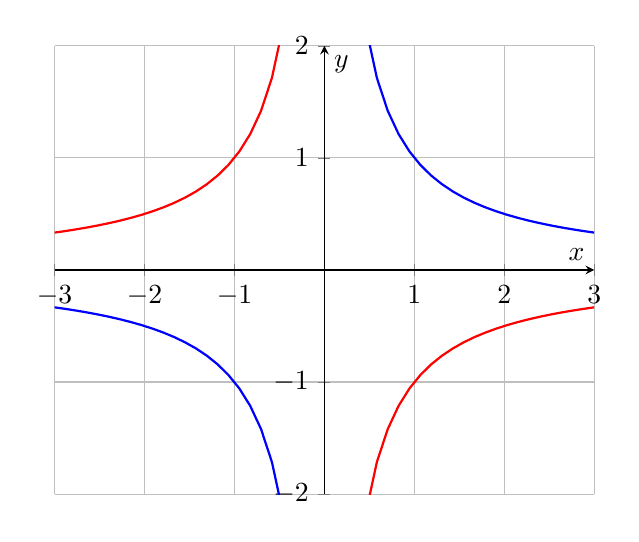
\begin{tikzpicture}
    \begin{axis}[
        grid=both,
        axis lines=middle,
        xmin=-3, xmax=3,
        ymin=-2, ymax=2,
        xlabel={$x$},
        ylabel={$y$},
        ]
        \addplot[blue, thick, domain=-3:-0.1] {1/x};
        \addplot[blue, thick, domain=0.1:3] {1/x};
        \addplot[red, thick, domain=3:0.1]{-1/x};
        \addplot[red, thick, domain=-0.1:-3]{-1/x};
    \end{axis}
\end{tikzpicture}
\end{minipage}
\hspace{1cm}
\begin{minipage}{0.4\textwidth}
\centering
\begin{tabular}{|c|c|c|c|}

$x$ & $\frac{1}{x}$ & $-\frac{1}{x}$ \\ 
\hline
-3 & -0.33 & -0.33 \\
\hline
-2 & -0.5 & -0.5 \\
\hline
-1 & -1 & -1 \\
\hline
1 & 1 & -1 \\
\hline 
2 & 0.5 & -0.5 \\
\hline
3 & 0.33 & -0.33 \\

\end{tabular}
\end{minipage}
\noindent
The reciprocal function $f(x) = \frac{1}{x}$ has \hl{two hyperbolas} in the 1st and 3rd quadrants. As $x$ approaches 0 from either side, $f(x)$ approaches $\pm\infty$. 
\subsubsection{End Behaviour}
\begin{align*}
    x \to -\infty, y=0^-\\
    x \to +\infty, y\to 0^+\\
    x \to 0^-, y \to-\infty\\
    x\to 0^+, y\to+\infty\\
    x\in (-\infty,0) \quad y \downarrow \\
    x > 0 \quad  y \downarrow \\
    x \in (0, +\infty) \quad y \downarrow 
\end{align*}

\subsubsection{Domain and Range}
\begin{equation*}
    D: \{x \in \mathbb{R} | x \neq 0\}, 
    R: \{y \in \mathbb{R} | y \neq 0\} 
\end{equation*}
\subsubsection*{Example 1:}
Solve for $f(x)=\frac{1}{-3x+5}$
\begin{enumerate}
\item[a)] State the domain and range.
\item[b)] Describe the behaviour of the function near the vertical asymptote.
\item[c)] Describe the end behaviour.
\item[d)] Sketch a graph of the function.
\end{enumerate}
\subsubsection*{Solution}
\begin{enumerate}
    \item[a)] \textbf{Domain \& Range}:
    The function \( f(x) = \frac{1}{-3x + 5} \) will be undefined when the denominator equals zero because division by zero is undefined. So, we solve for \( x \):
    \[ -3x + 5 = 0 \]
    \[ -3x = -5 \]
    \[ x = \frac{5}{3} \]
    So, the domain of the function is all real numbers except \( x = \frac{5}{3} \). 
    The range is $R: \{y \in \mathbb{R} | y \neq 0\}$
    
    \item[b)] \textbf{Behaviour near the vertical asymptote}:
    The vertical asymptote occurs when the denominator approaches zero, which in this case is \( x = \frac{5}{3} \). Near this point, the function behaves similarly to \( \frac{1}{x} \), approaching positive or negative infinity depending on whether \( x \) approaches \( \frac{5}{3} \) from the left or the right, respectively.
    
    \item[c)] \textbf{End behaviour}:
    As \( x \) approaches positive or negative infinity, \( f(x) \) approaches zero. This is because the term \( -3x \) dominates the function as \( x \) becomes very large in magnitude, making the entire fraction approach zero.
    
    \item[d)] \textbf{Sketch of the graph}:
    The graph will be a hyperbola with a vertical asymptote at \( x = \frac{5}{3} \) and approaching the x-axis as \( x \) approaches positive or negative infinity.
    \begin{figure}[ht]
    \centering
    \includegraphics[width=0.9\textwidth]{imgs/graph(1_3x+5).png}
    \end{figure}
    \\
    $x\to \frac{5}{3}^-, y\to \infty$, $x\in (-\infty,\frac{5}{3})$ increase\\
    $x \to \frac{5}{3}^+, y\to -\infty$, $x\in(\frac{5}{3}, +\infty)$ increase
\end{enumerate}

\subsubsection*{Example 2:}
Solve for $f(x)=\frac{1}{(x+1)(x-3)}$
\begin{enumerate}
\item[a)] State the domain and range.
\item[b)] Describe the behaviour of the function near the vertical asymptote.
\item[c)] Describe the end behaviour.
\item[d)] Sketch a graph of the function.
\end{enumerate}
\subsubsection*{Solution:}

\begin{enumerate}
    \item[a)] \text{Domain and Range:}
    The function \( f(x) = \frac{1}{(x+1)(x-3)} \) is undefined at \( x = -1 \) and \( x = 3 \).     So, the domain of the function is all real numbers except \( x = -1 \) and \( x = 3 \). The range is all real numbers except when \( f(x) \) equals zero.
    
    \item[b)] \text{Behaviour near the vertical asymptotes}:
    Near \( x = -1 \) and \( x = 3 \), the function behaves like \( \frac{1}{x} \), approaching infinity as \( x \) approaches these points.
    
    \item[c)] \text{End behaviour }
    As \( x \) tends to positive or negative infinity, \( f(x) \) approaches zero due to the dominance of \( (x+1) \) and \( (x-3) \) in the denominator.
    \item[d)] \text{Sketch of the graph:}
    \begin{figure}[ht]
    \centering
    \includegraphics[width=0.9\textwidth]{imgs/graph(1_x+1_x-3).png}
    \end{figure}
\end{enumerate}
$x\to -1^-, y\to +\infty \quad x\to 3^-, y\to -\infty$ \quad $x\in(-\infty, -1)(3, +\infty) y >0$ \\
$x\to -1^+, y \to +\infty \quad x\to 3^+, y\to +\infty$ \quad $x\in(-1,3) y< 0$

\subsection{Reciprocals of Quadratic Functions}
A quadratic function has the form f (x) = ax2 + bx + c in
standard form, where a, b and c are real coefficients.\\
What does the graph of the reciprocal of a quadratic look
like?\\
There are three cases to consider, depending on the
factorability of the quadratic.
\subsubsection{Asymptotes}
Vertical asymptotes occur when the denominator of a
rational expression is zero. Thus, the roots of a quadratic expression in the denominator correspond to any vertical asymptotes.\\
Since a quadratic may have zero, one or two real roots, the
reciprocal of a quadratic may have zero, one or two vertical
asymptotes.\\

Like reciprocals of linear functions, horizontal asymptotes can
be determined by dividing each term by the highest power,
then evaluating as $x\to\infty$.
\subsection*{Example:}
Determine the equations of any asymptotes for
$$
f(x)=\frac{1}{x^2-4} \text {. }
$$

After factoring, $f(x)=\frac{1}{(x-2)(x+2)}$.
There are two vertical asymptotes: one with equation $x=-2$, and the other $x=2$.
Divide the expression by $x^2$ and let $x \rightarrow \infty$.
$$
\begin{aligned}
\frac{\frac{1}{x^2}}{\frac{x^2}{x^2}-\frac{4}{x^2}} & =\frac{0}{1-0} \\
& =0
\end{aligned}
$$
\subsection*{Asymptotes}

\begin{minipage}{0.6\textwidth}
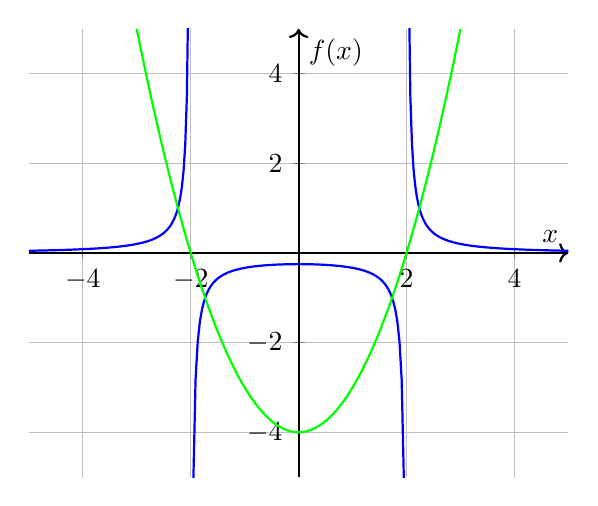
\begin{tikzpicture}
\begin{axis}[
    xlabel={$x$},
    ylabel={$f(x)$},
    xmin=-5, xmax=5,
    ymin=-5, ymax=5,
    axis lines=center,
    axis line style=->,
    legend pos=north west,
    samples=100,
    grid=major,
    thick
]
\addplot[blue,domain=-5:-2.01] {1/(x^2 - 4)};
\addplot[blue,domain=-1.99:1.99] {1/(x^2 - 4)};
\addplot[blue,domain=2.01:5] {1/(x^2 - 4)};
\addplot[green, domain=-3:3]{x^2-4};
\end{axis}
\end{tikzpicture}
\end{minipage}%
\begin{minipage}{0.4\textwidth}
$f(x)$ is symmetric about the same axis as $g(x)$. A local maximum occurs on $f(x)$ where there is a local minimum on $g(x)$.
\end{minipage}
\subsubsection{Intercepts}
As with any function, the f(x)-intercept can be found by
substituting $x = 0$ into its equation.\\
x-intercepts will occur when the numerator evaluates to zero.
If the reciprocal of a quadratic has the form
$$f(x) = \frac{1}{ax^2 + bx + c},$$ then there will always be a horizontal
asymptote at f (x) = 0.
Verifying the last example, the f (x)-intercept is at $\frac{1}{0^-4}=\frac{1}{4}$ and there are no x-intercepts.

\subsubsection{Minima/Maxima}
Since functions of the form $$f(x) = \frac{1}{ax^2 + bx + c},$$
have line symmetry, any minimum or maximum point will occur
halfway between the two vertical asymptotes.\\
Substituting in this middle value allows us to determine the
coordinate where there is a local min/max.
In the previous example, the vertical asymptotes were at $x = -2$ and $x = 2$.
Therefore, a local minimum or maximum will occur when\\
\begin{equation*}
    x=\frac{-2+2}{2}=0 \quad \text{or at} \quad \left(0, -\frac{1}{4}\right)
\end{equation*}
\subsection{Rational Functions of the Form $f(x)\frac{ax+b}{cx+d}$}
\textbf{Recall that a rational function is a ratio of two polynomial functions, $p(x)$ and $q(x)$, such that $f(x) = \frac{p(x)}{q(x)}$.} Since $q(x) \neq 0$, there will often be some form of discontinuity, such as an asymptote or a hole. In this section, we will investigate rational functions that have the form $f(x) = \frac{ax + b}{cx + d}$. Such functions have predictable properties, making them easy to graph.

\subsubsection*{Example}
\textbf{Graph the function $f(x) = \frac{x + 4}{x - 2}$ and describe its properties.} There is a vertical asymptote at $x = 2$. Dividing each term by $x$ to find the equation of the horizontal asymptote:
\[
\frac{x}{x} + \frac{4}{x} \div \frac{x}{x} - \frac{2}{x} = \frac{1 + 0}{1 - 0} = 1
\]
A horizontal asymptote occurs at $f(x) = 1$. The $x$-intercept is at $x = -4$ and the $f(x)$-intercept is at $-2$.

\begin{center}
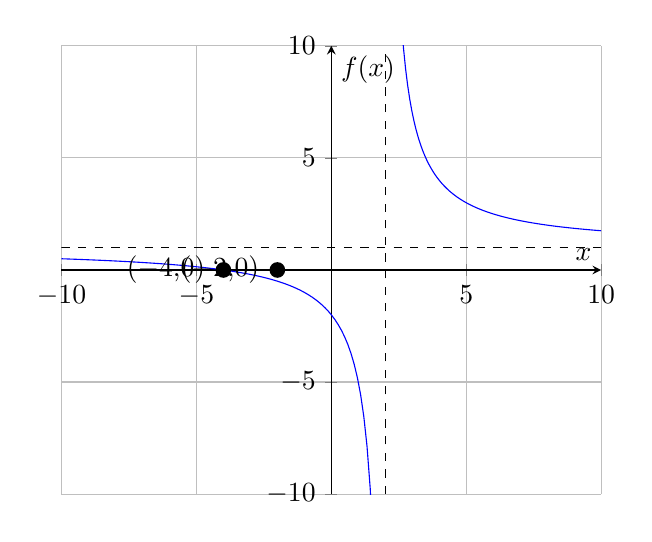
\begin{tikzpicture}
\begin{axis}[
    axis lines=middle,
    xlabel={$x$},
    ylabel={$f(x)$},
    xmin=-10, xmax=10,
    ymin=-10, ymax=10,
    xtick={-10,-5,...,10},
    ytick={-10,-5,...,10},
    grid=both,
    ]
    \addplot[domain=-10:1.8,blue,samples=100] {(x + 4)/(x - 2)};
    \addplot[domain=2.2:10,blue,samples=100] {(x + 4)/(x - 2)};
    \draw[dashed] (2,-10) -- (2,10);
    \draw[dashed] (-10,1) -- (10,1);
    \node[label={180:{($-4$,0)}},circle,fill,inner sep=2pt] at (-4,0) {};
    \node[label={180:{($-2$,0)}},circle,fill,inner sep=2pt] at (-2,0) {};
\end{axis}
\end{tikzpicture}
\end{center}

\subsubsection{Putting it Together}
To determine the function's behavior to the right of the vertical asymptote, test values of $x$ greater than $2$.

\subsubsection{Symmetry}
$f(4) = 4$ and $f(8) = 2$, resulting in a symmetric graph about the asymptotes.

\subsubsection{Complete Graph}
A complete graph of $f(x)$ confirms the symmetry.

\subsubsection*{Example 2}
\textbf{Graph the function $f(x) = \frac{2x - 1}{x + 1}$.} There is a vertical asymptote at $x = -1$. Dividing each term by $x$ to find the equation of the horizontal asymptote:
\[
\frac{2x}{x} - \frac{1}{x} \div \frac{x}{x} + \frac{1}{x} = \frac{2 - 0}{1 + 0} = 2
\]
A horizontal asymptote occurs at $f(x) = 2$. The $x$-intercept is at $\frac{1}{2}$ and the $f(x)$-intercept is at $-1$.

\begin{center}
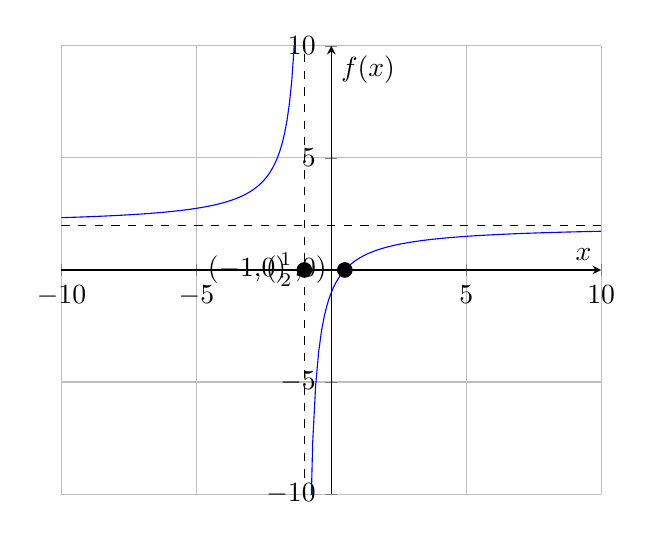
\begin{tikzpicture}
\begin{axis}[
    axis lines=middle,
    xlabel={$x$},
    ylabel={$f(x)$},
    xmin=-10, xmax=10,
    ymin=-10, ymax=10,
    xtick={-10,-5,...,10},
    ytick={-10,-5,...,10},
    grid=both,
    ]
    \addplot[domain=-10:-1.2,blue,samples=100] {(2*x - 1)/(x + 1)};
    \addplot[domain=-0.8:10,blue,samples=100] {(2*x - 1)/(x + 1)};
    \draw[dashed] (-1,-10) -- (-1,10);
    \draw[dashed] (-10,2) -- (10,2);
    \node[label={180:{($\frac{1}{2}$,0)}},circle,fill,inner sep=2pt] at (0.5,0) {};
    \node[label={180:{($-1$,0)}},circle,fill,inner sep=2pt] at (-1,0) {};
    
\end{axis}
\end{tikzpicture}
\end{center}

\subsubsection{Comparison}
Comparing the graphs of $f(x) = \frac{x+4}{x-2}$, $g(x) = \frac{x+3}{x-2}$, and $h(x) = \frac{x+2}{x-2}$.

\subsubsection{Properties}
All three functions have the form $\frac{ax + b}{cx + d}$. As the value of $b$ increases, the function is stretched further from the asymptotes. The value of $b$ has no effect on the vertical and horizontal asymptotes.

\subsubsection*{Example 3}
\textbf{Determine the equation of a rational function with the following features:}
\begin{itemize}
    \item A vertical asymptote at $x = 3$.
    \item A horizontal asymptote at $f(x) = 2$.
    \item An $x$-intercept at $x = 1$.
\end{itemize}
Since a vertical asymptote occurs at $x = 3$, let the denominator be $x - 3$. In order for a horizontal asymptote to occur at $f(x) = 2$, and since $c = 1$, the value of $a$ must be $2$, since $a/c = 2/1 = 2$. The $x$-intercept occurs when the numerator is zero, or $2x + b = 0$. Isolating $x$, this becomes $x = -\frac{b}{2}$. Since the $x$-intercept is $1$, $-\frac{b}{2} = 1$, or $b = -2$. Thus, a possible equation is $f(x) = \frac{2x - 2}{x - 3}$.


\subsection{Rational equations and inequalities}
To solve equations involving rational expressions, we have the freedom to clear out fractions before proceeding. After multiplying both sides by the common denominator, we are left with a polynomial equation.

\subsubsection*{Example:}
Solve the equation $\frac {2}{x} + \frac {3x}{x+1} = 4.$
\subsubsection*{Solution }
The common denominator is x(x+1). We multiply both sides by x(x+1)
 to clear out the fractions.
\begin{align*} 
      \frac{2}{x} + \frac{3x}{x+1} &= 4  \\
      x(x+1) \left( \frac{2}{x} + \frac{3x}{x+1} \right) &= x(x+1) ( 4 )\\
      x(x+1) \cdot \frac{2}{x}  + x(x+1) \cdot \frac{3x}{x+1} &= 4x(x+1)\\
      2(x+1) + 3x(x) &= 4x^2 + 4x\\
      3x^2 + 2x + 2 &= 4x^2 + 4x\\
      x^2 + 2x - 2 &= 0.
    \end{align*}
The quadratic formula gives solutions as $\displaystyle x = \dfrac {-2 \pm \sqrt {12}}{2} = -1 \pm \sqrt {3}$\\

If we look back at the original equation, we notice that there are some numbers that we are not allowed to plug in for \(x\). When \(x=0\) or \(x=-1\), the left-hand side of the equation is not defined due to a division by zero issue. Since neither \(-1 + \sqrt{3}\) nor \(-1 - \sqrt{3}\) have such an issue, they are both solutions.
\subsubsection{Inequalities}
When faced with nonlinear inequalities, such as those involving general rational functions, we make use of a sign chart. The inequality in the following example is not given in factored form, so we have some work to do.

\subsubsection*{Example}
Solve the inequality $\displaystyle x^2 + 5x \leq -10 -\dfrac {16}{x-2}$
\subsubsection*{Solution}
We’ll begin by moving everything to one side, then combining them all together into a single fraction.

\begin{align*} 
         x^2 + 5x &\leq -10 -\dfrac{16}{x-2}\\
      x^2 + 5x +10 +\dfrac{16}{x-2} &\leq 0\\
      \left(x^2+5x+10\right) \cdot \left(\dfrac{x-2}{x-2}\right) +\dfrac{16}{x-2} &\leq 0\\
      \dfrac{x^3+3x^2-20}{x-2} + \dfrac{16}{x-2} &\leq 0\\    
      \dfrac{x^3+3x^2-4}{x-2} &\leq 0\\
      \dfrac{(x-1)(x+2)^2}{x-2} &\leq 0
    \end{align*}
    Now that the inequality is in a better form for us to work with, we’ll build a sign chart like we did in the last example.

    \begin{figure}[ht]
    \centering
    \includegraphics[width=0.9\textwidth]{imgs/graph figure.png}
    \end{figure}
We see from the chart that $\displaystyle \frac{(x-1)(x+2)^2}{x-2}$ will be negative in $(1,2)$. At $x=-2$ and $x=1$ it is zero. The solution is then: $(-2) \cup [1,2)$.
\newpage
\subsection{Making Connections With Rational Functions and Equation}
\textcolor{red}{Special cases} occur when a factored rational function has the exact same bracket in both the numerator and denominator. In this case, the
bracket would be crossed out on both the top and bottom and a statement reflecting a hole at that point would be made.

\section*{Resources}
\begin{itemize}
    \item \href{https://ximera.osu.edu/calcwithreview/calculusWithReview/rationalFunctions/digInRationalEqIneq}{Rational equations and inequalities}
    \item \href{https://www.andrews.edu/~rwright/Precalculus-RLW/Text/02-07.html#:~:text=A%20vertical%20asymptote%20of%20a,inputs%20approach%20%E2%88%9E%20or%20%E2%80%93%E2%88%9E.}{Veritcal and horizontal asymptotes }
\end{itemize}
\newpage

\section{Unit 4}
\subsection{Radian Measure}
If you draw a circle with center $O$ and radius $r$, and you draw two radii $OA$ and $OB$, then you can define length $AB$ as an arc $a$ and angle $AOB$ as $\theta$.
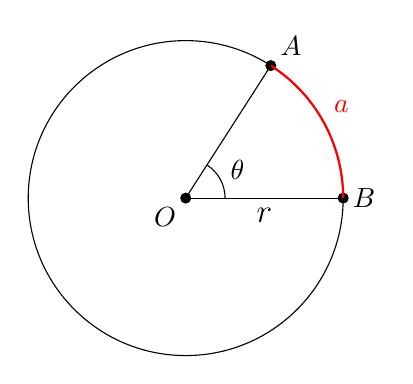
\begin{tikzpicture}
    % Define radius
    \def\radius{2cm}

    % Draw circle
    \draw (0,0) circle (\radius);
    
    % Define center, points A and B
    \coordinate[label=below left:$O$] (O) at (0,0);
    \coordinate[label=above right:$A$] (A) at (57.2958:\radius);
    \coordinate[label=right:$B$] (B) at (0:\radius);
    
    % Draw points
    \foreach \point in {O, A, B}
        \fill (\point) circle (2pt);
    
    % Draw arc AB
    \draw[thick, red] (A) arc (57.2958:0:\radius) node[midway, above right] {$a$};

    \draw (B)--(O) node[midway, below, font=\large] {$r$};

    \draw (O)--(A);
    
    % Draw and label angle AOB with theta
    \pic[draw, "$\theta$", angle eccentricity=1.5] {angle = B--O--A};
\end{tikzpicture}

The Radian Measure is way to express an angle as a ratio. The radian measure of an angle $\theta$ is defined as the length of an arc ($a$) divided by the radius ($r$). 
$$\theta=\frac{a}{r}$$

One radius is when the angle of the arc is equal to the radius. What about a full rotation?

Well, we know that the circumstance of a circle is $2\pi r$, so we can substitute this arc length of a full rotation into the definition of a radian.
$$\theta = \frac{2\pi r}{r}=2 \pi rad \approx 6.28 rad$$

When using angles in radians, it is convention to drop the units. We can conclude that a full rotation of a circle, then, is $2\pi$

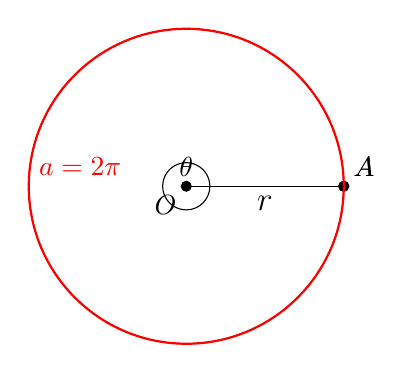
\begin{tikzpicture}
    \def\radius{2cm}
    \draw (0,0) circle (\radius);
    \draw (0,0) circle (0.3cm) node[above] {$\theta$};
    \coordinate[label=below left:$O$] (O) at (0,0);
    \coordinate[label=above right:$A$] (A) at (0:\radius);
    \coordinate[label=above right:$A$] (B) at (360:\radius);
    \foreach \point in {O, A, B}
    \fill (\point) circle (2pt);
    \draw[thick, red] (A) arc (360:0:\radius) node[midway, above right] {$a=2\pi$};
    \draw (A)--(O) node[midway, below, font=\large] {$r$};
\end{tikzpicture}

\subsubsection{Radian-Degree Conversion}
\begin{align*}
&\text{Radian} \longrightarrow \text{Degree} \left(\frac{\pi}{180^{\circ}}\right)\\
&\text{Radian} \longleftarrow \text{Degree} \left(\frac{180^{\circ}}{\pi}\right)
\end{align*}

\newpage
\subsection{Trig Ratios and Special Angles}
The triangles found in a geometry set are a $45^{\circ}-45^{\circ}-90^{\circ}$ triangle and a $30^{\circ}-60^{\circ}-90^{\circ}$ triangle. These triangles can be used to construct similar triangles with 
the same special relationships among the sides.

\begin{figure}[ht]
    \centering
    \includegraphics[width=0.5\textwidth]{imgs/special trigs.PNG}
\end{figure}

\begin{align*}
&\sin \left(\frac{2 \pi}{3}\right) = \frac{\sqrt{3}}{2}, \quad &
&\csc \left(\frac{2 \pi}{3}\right) = \frac{2}{\sqrt{3}}, \\
&\cos \left(\frac{2 \pi}{3}\right) = -\frac{1}{2}, \quad &
&\sec \left(\frac{2 \pi}{3}\right) = -2, \\
&\tan \left(\frac{2 \pi}{3}\right) = -\sqrt{3}, \quad &
&\cot \left(\frac{2 \pi}{3}\right) = -\frac{1}{\sqrt{3}}
\end{align*}


\begin{table}[htbp]
\centering
\caption{Special Angles and Trigonometric Ratios}
\label{tab:special_angles}
\begin{tabular}{|c|c|c|c|c|c|c|c|}
\hline
Angle & Degrees & Radians & \( \sin \theta \) & \( \cos \theta \) & \( \tan \theta \) & \( \csc \theta \) & \( \sec \theta \) \\ \hline
\( 0^\circ \) & \( 0^\circ \) & \( 0 \) & \( 0 \) & \( 1 \) & \( 0 \) & undefined & \( 1 \) \\ \hline
\( 30^\circ \) & \( 30^\circ \) & \( \frac{\pi}{6} \) & \( \frac{1}{2} \) & \( \frac{\sqrt{3}}{2} \) & \( \frac{1}{\sqrt{3}} \) & \( 2 \) & \( \frac{2}{\sqrt{3}} \) \\ \hline
\( 45^\circ \) & \( 45^\circ \) & \( \frac{\pi}{4} \) & \( \frac{\sqrt{2}}{2} \) & \( \frac{\sqrt{2}}{2} \) & \( 1 \) & \( \sqrt{2} \) & \( \sqrt{2} \) \\ \hline
\( 60^\circ \) & \( 60^\circ \) & \( \frac{\pi}{3} \) & \( \frac{\sqrt{3}}{2} \) & \( \frac{1}{2} \) & \( \sqrt{3} \) & \( \frac{2}{\sqrt{3}} \) & \( 2 \) \\ \hline
\( 90^\circ \) & \( 90^\circ \) & \( \frac{\pi}{2} \) & \( 1 \) & \( 0 \) & undefined & \( 1 \) & undefined \\ \hline
\end{tabular}
\end{table}
\subsubsection*{Example}
Determine exact values of the six trigonometric ratios for an angle of $\frac{3 \pi}{4}$
\begin{align*}
&\sin \left(\frac{3\pi}{4}\right) = \frac{\sqrt{2}}{2}, \quad \csc \left(\frac{3\pi}{4}\right) = \sqrt{2}, \\
&\cos \left(\frac{3\pi}{4}\right) = -\frac{\sqrt{2}}{2}, \quad \sec \left(\frac{3\pi}{4}\right) = -\sqrt{2}, \\
&\tan \left(\frac{3\pi}{4}\right) = -1, \quad \cot \left(\frac{3\pi}{4}\right) = -1.
\end{align*}

You can use the unit circle and special triangles to determine exact values for the trigonometric ratios of the special angles $0, \frac{\pi}{6}, \frac{\pi }{4}, \frac{\pi }{3}$ and $\frac{ \pi}{2}$

\newpage
\section*{Unit Circle }
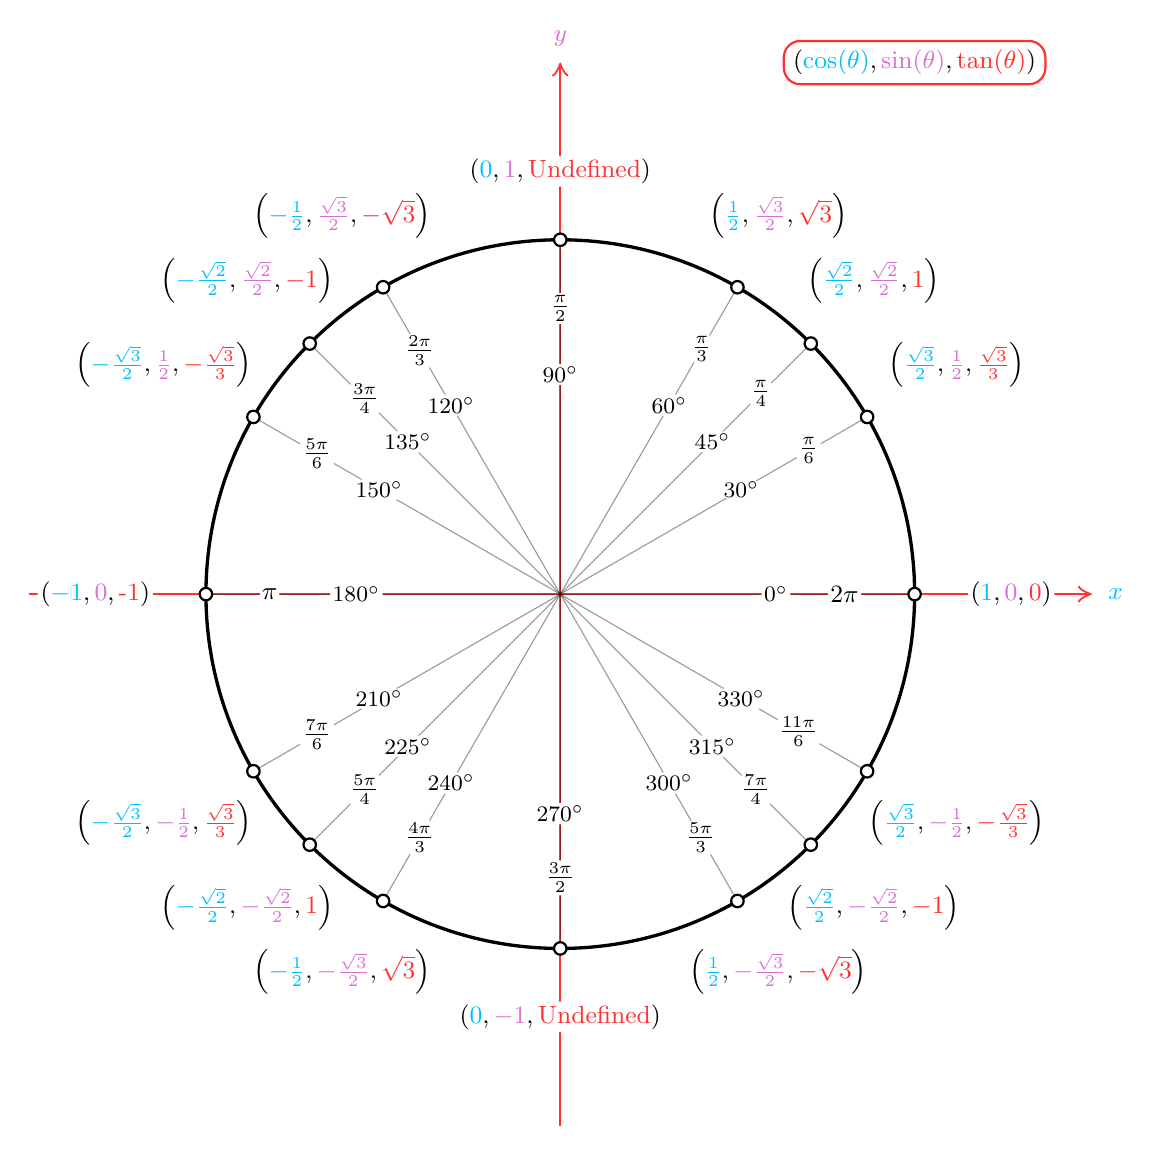
\begin{tikzpicture}[scale=4.5, font=\small]
    \definecolor{r}{HTML}{ff3030}
    \definecolor{b}{HTML}{00bfff}
    \definecolor{o}{HTML}{DA70D6}
    \def\angles{
        0/2\pi/1/0/0,
        30/\frac{\pi}{6}/\frac{\sqrt{3}}{2}/\frac{1}{2}/\frac{\sqrt{3}}{3},
        45/\frac{\pi}{4}/\frac{\sqrt{2}}{2}/\frac{\sqrt{2}}{2}/1,
        60/\frac{\pi}{3}/\frac{1}{2}/\frac{\sqrt{3}}{2}/\sqrt{3},
        90/\frac{\pi}{2}/0/1/\text{Undefined},
        120/\frac{2\pi}{3}/-\frac{1}{2}/\frac{\sqrt{3}}{2}/-\sqrt{3},
        135/\frac{3\pi}{4}/-\frac{\sqrt{2}}{2}/\frac{\sqrt{2}}{2}/-1,
        150/\frac{5\pi}{6}/-\frac{\sqrt{3}}{2}/\frac{1}{2}/-\frac{\sqrt{3}}{3},
        180/\pi/-1/0/\text{-1},
        210/\frac{7\pi}{6}/-\frac{\sqrt{3}}{2}/-\frac{1}{2}/\frac{\sqrt{3}}{3},
        225/\frac{5\pi}{4}/-\frac{\sqrt{2}}{2}/-\frac{\sqrt{2}}{2}/1,
        240/\frac{4\pi}{3}/-\frac{1}{2}/-\frac{\sqrt{3}}{2}/\sqrt{3},
        270/\frac{3\pi}{2}/0/-1/\text{Undefined},
        300/\frac{5\pi}{3}/\frac{1}{2}/-\frac{\sqrt{3}}{2}/-\sqrt{3},
        315/\frac{7\pi}{4}/\frac{\sqrt{2}}{2}/-\frac{\sqrt{2}}{2}/-1,
        330/\frac{11\pi}{6}/\frac{\sqrt{3}}{2}/-\frac{1}{2}/-\frac{\sqrt{3}}{3}
    }
    \begin{scope}[every node/.style={inner sep=1pt, outer sep=0pt}]
        \foreach \a/\at/\x/\y/\t in \angles {
            \begin{pgfinterruptboundingbox}
                \node (x) at (\a : 1.15) [anchor=\a-180] {\phantom{$\textstyle\left({\color{b} \x}, {\color{o} \y}, {\color{r} \t}\right)$}};
                \clip [rounded corners] (x.south west) rectangle (x.north east) (-1.6, -1.6) -- (1.6, -1.6) -- (1.6, 1.6) -- (-1.6, 1.6) -- cycle;
                \node (x) at (\a : 0.85) [anchor=\a] {\phantom{$\textstyle\at$}};
                \clip [rounded corners] (x.south west) rectangle (x.north east) (-1.6, -1.6) -- (1.6, -1.6) -- (1.6, 1.6) -- (-1.6, 1.6) -- cycle;
                \node (x) at (\a : 0.65) [anchor=\a, font=\footnotesize] {\phantom{$\textstyle\a^\circ$}};
                \clip [rounded corners] (x.south west) rectangle (x.north east) (-1.6, -1.6) -- (1.6, -1.6) -- (1.6, 1.6) -- (-1.6, 1.6) -- cycle;
                \clip (\a : 1) circle [radius=.5pt] (-1.6, -1.6) -- (-1.6, 1.6) -- (1.6, 1.6) -- (1.6, -1.6) -- cycle;
            \end{pgfinterruptboundingbox}
        }

        \draw [r, thick] (-1.5, 0) edge [-{Classical TikZ Rightarrow[length=5pt, width=6pt]}] (1.5, 0) node at (1.5, 0) [right=5pt] {$\textstyle\color{b} x$}
        (0, -1.5) edge [-{Classical TikZ Rightarrow[length=5pt, width=6pt]}] (0, 1.5) node at (0, 1.5) [above=5pt] {$\textstyle\color{o} y$};
        \draw [very thick] (0, 0) circle [radius=1];

        \foreach \a/\at/\x/\y/\t in \angles { \draw [opacity=.4] (0, 0) -- (\a : 1); }
    \end{scope}

    \scoped [every node/.style={inner sep=1pt, outer sep=0pt}] {
        \foreach \a/\at/\x/\y/\t in \angles {
            \node at (\a : 1.15) [anchor=\a-180, rounded corners] {$\textstyle\left({\color{b} \x}, {\color{o} \y}, {\color{r} \t}\right)$};
            \node at (\a : 0.85) [anchor=\a, rounded corners] {$\textstyle\at$};
            \node at (\a : 0.65) [anchor=\a, rounded corners, font=\footnotesize] {$\textstyle\a^\circ$};
            \draw [thick] (\a : 1) circle [radius=.5pt];
        }
    }

    \node at (1, 1.5) [thick, draw=r, rounded corners=6pt] {$\textstyle\left({\color{b} \cos(\theta)}, {\color{o} \sin(\theta)}, {\color{r} \tan(\theta)}\right)$};
\end{tikzpicture}
\newpage 

\subsection{Equivalent Trigonometric Expression}
\textbf{Definition: Equivalent Trigonometric Expressions}

Equivalent trigonometric expressions refer to different algebraic representations of the same trigonometric function or identity. Two trigonometric expressions are considered equivalent if they produce the same value for all possible inputs (angles).

For example, consider the Pythagorean identity:
\[
\sin^2(x) + \cos^2(x) = 1
\]
This equation demonstrates that the sum of the squares of the sine and cosine of an angle \( x \) is always equal to 1. Thus, the expressions \( \sin^2(x) + \cos^2(x) \) and \( 1 \) are equivalent.

Similarly, expressions such as \( \tan(x) \) and \( \frac{\sin(x)}{\cos(x)} \) are equivalent, as they represent the same trigonometric function, tangent.

Understanding equivalent trigonometric expressions is crucial for simplifying complex trigonometric equations, identities, and functions, as well as for solving trigonometric equations efficiently.

\begin{figure}[ht]
    \centering
    \includegraphics[width=0.5\textwidth]{imgs/circle equivalent.PNG}
\end{figure}
\begin{center}
\centering
$$
\begin{array}{|c|c|c|c|}
\hline \sin \left(\frac{\pi}{2}+\theta\right)=\cos \theta & \csc \left(\frac{\pi}{2}+\theta\right)=\sec \theta & \sin \left(\frac{\pi}{2}-\theta\right)=\cos \theta & \csc \left(\frac{\pi}{2}-\theta\right)=\sec \theta \\
\hline \cos \left(\frac{\pi}{2}+\theta\right)=-\sin \theta & \sec \left(\frac{\pi}{2}+\theta\right)=-\csc \theta & \cos \left(\frac{\pi}{2}-\theta\right)=\sin \theta & \sec \left(\frac{\pi}{2}-\theta\right)=\csc \theta \\
\hline \tan \left(\frac{\pi}{2}+\theta\right)=-\cot \theta & \cot \left(\frac{\pi}{2}+\theta\right)=-\tan \theta & \tan \left(\frac{\pi}{2}-\theta\right)=\cot \theta & \cot \left(\frac{\pi}{2}-\theta\right)=\tan \theta \\
\hline
\end{array}
$$
\end{center}

\subsection{Compound Angle Formulas}

The compound angle formulas are as follows:
\begin{align*}
& \sin(x+y)=\sin x \cos y+\cos x \sin y\\
& \sin (x-y)=\sin x\cos y-\cos-\cos x \sin y\\
& \cos(x+y)=\cos x\cos y -\sin x \sin y\\
&\cos (x-y)=\cos x \cos y+\sin x \sin y
\end{align*}
\subsubsection{Proof: }
\begin{figure}[ht]
    \centering
    \includegraphics[width=0.9\textwidth]{imgs/proof.png}
\end{figure}

\subsubsection{Addition Formula for Sine}
Recall the cofunction identities $\sin x=\cos \left(\frac{\pi}{2}-x\right)$ and $\cos x=\sin \left(\frac{\pi}{2}-x\right)$.
Apply these and the subtraction formula for cosine.
$$
\begin{aligned}
\sin (x+y) & =\cos \left[\frac{\pi}{2}-(x+y)\right] \quad \text{Apply a cofunction identity.}\\
& =\cos \left[\left(\frac{\pi}{2}-x\right)-y\right] \quad \text{Regroup the terms in the argument.}\\
& =\cos \left(\frac{\pi}{2}-x\right) \cos y+\sin \left(\frac{\pi}{2}-x\right) \sin y \quad \text{Apply the subtraction formula for cosine.}\\
& =\sin x \cos y+\cos x \sin y \quad \text{Apply cofunction identities.}
\end{aligned}
$$
\subsubsection{Subtraction Formula for Sine}
The subtraction formula for sine can be derived from the addition formula for sine, following the approach used for the subtraction formula for cosine.
$$
\begin{aligned}
& \sin (x+(-y))=\sin x \cos (-y)+\cos x \sin (-y) \quad \text { Substitute }-y \text { for } y \\
& \sin (x-y)=\sin x \cos y+\cos x(-\sin y) \\
& \sin (x-y)=\sin x \cos y-\cos x \sin y
\end{aligned}
$$

\subsubsection*{Example}
The angles $\alpha$ and $\theta$ are located in the FIRST quadrant. If $\sin\theta=\frac{2}{3}$ and $\sin \alpha=\frac{1}{2}$, find $\cos(\theta, \alpha)$

\subsubsection*{Solution}
\begin{align*}
    \cos(\theta- \alpha)&=\cos \theta \cos \alpha+\sin \thet  \sin \alpha\\
\end{align*}
We are told that these are first quarter  so that we know the signs of all the trig ratios using CAST rule. Other than that we can use right angle to find all other trig ratios for the two angles
\begin{align*}
    &=\left(\frac{\sqrt{5}}{3}\right)\left(\frac{\sqrt{3}}{2}\right)+\left(\frac{2}{3}\right)\left(\frac{1}{2}\right)\\
    &=\frac{\sqrt{15}}{6}+\frac{2}{6}\\
    &=\frac{\sqrt{15}+2}{6}
\end{align*}
\newpage

\subsection{Prove Trig Identities }


    \textit{Quotient Identity :} $\tan \theta=\frac{\sin \theta}{\cos \theta}$

\textit{Pythagorean Identity:} $\sin ^2 \theta+\cos ^2 \theta=1$ (from the unit circle)

\textit{Reciprocal Identities :}
$$
\begin{array}{ll}
\csc \theta=\frac{1}{\sin \theta} ; \quad \sin \theta=\frac{1}{\csc \theta} \\
\sec \theta=\frac{1}{\cos \theta} ; \quad \cos \theta=\frac{1}{\sec \theta} \\
\tan \theta=\frac{1}{\cot \theta} ; \quad \cot \theta=\frac{1}{\tan \theta}
\end{array}
$$

\textit{Compound Angle Formulas:}
$$
\begin{aligned}
\sin (x+y) & =\sin x \cos y+\cos x \sin y \\
\sin (x-y) & =\sin x \cos y-\cos x \sin y \\
\cos (x+y) & =\cos x \cos y-\sin x \sin y \\
\cos (x-y) & =\cos x \cos y+\sin x \sin y
\end{aligned}
$$
\textbf{Reciprocal of Trigonometry}
  \begin{spreadlines}{1.5ex}
    \begin{alignat*}{2}
      \csc(x) & = \tfrac 1 {\sin(x)}, \quad & \tan(x) & = \tfrac {\sin(x)} {\cos(x)} \\
      \sec(x) & = \tfrac 1 {\cos(x)}, \quad & \cot(x) & = \tfrac {\cos(x)} {\sin(x)}
    \end{alignat*}
  \end{spreadlines}
\subsection{Applying the Basic Identities}
When you prove trig identities, you are trying to do anything you can with the known trig identities in order to transform the two sides and make them look like each other.\\


You may need to work on BOTH sides of the equal sign, but start first with the side that looks the most complicated. Generally you want to take complicated and make it look more simple.\\


It is important the a for each step along the way, you state what identity or math operation you have used.

\subsubsection{Exercises}  
\begin{enumerate}
    \item[a)] Prove $\frac{1+\tan x}{1+\cot x}-\frac{1-\tan x}{\cot x-1}$ 
    \item[b)] Prove $\csc 2x+\cot 2x=\cot x$ 
\end{enumerate}
\newpage 


\section{Unit 5}
\subsection{Graphing Trig Functions $\sin x$ \& $\csc x$ and $\cos x$ \& $\csc x$}
In this section, we will be relating the features of $\sin x$ and $\cos x$ to their reciprocals. You will notice that these reciprocals relate to the original function similar to linear reciprocals and quadratic reciprocals.

(insert table of values for $\sin x$ and $\csc x$)

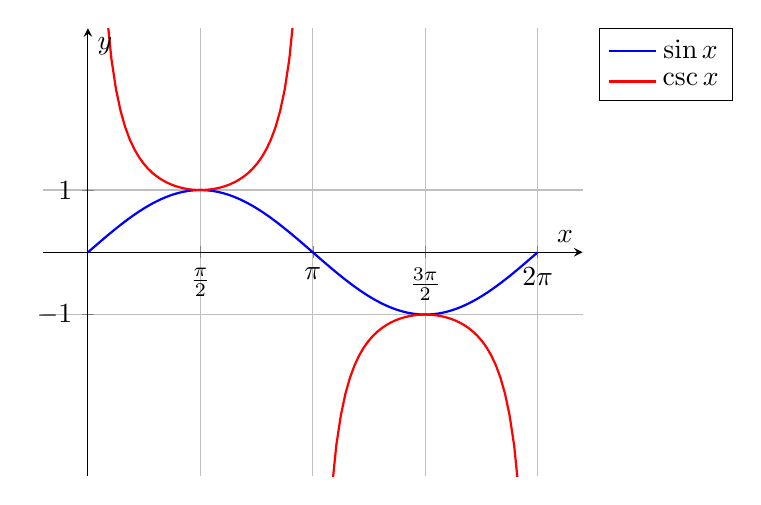
\begin{tikzpicture}
    \begin{axis}[
        domain=0:2*pi,
        samples=100,
        axis lines=middle,
        xlabel=$x$, ylabel=$y$,
        xtick={0, pi/2, pi, 3*pi/2, 2*pi},
        xticklabels={$0$, $\frac{\pi}{2}$, $\pi$, $\frac{3\pi}{2}$, $2\pi$},
        ytick={-1, 1},
        ymin=-3, ymax=3,
        grid=both,
        legend pos=outer north east,
        enlargelimits=true,
    ]
    \addplot [blue, thick] {sin(deg(x))};
    \addplot [red, thick, domain=0.01:pi-0.01, samples=50] {1/sin(deg(x))};
    \addplot [red, thick, domain=pi+0.01:2*pi-0.01, samples=50] {1/sin(deg(x))};
    \legend{$\sin x$, $\csc x$}
    \end{axis}
\end{tikzpicture}

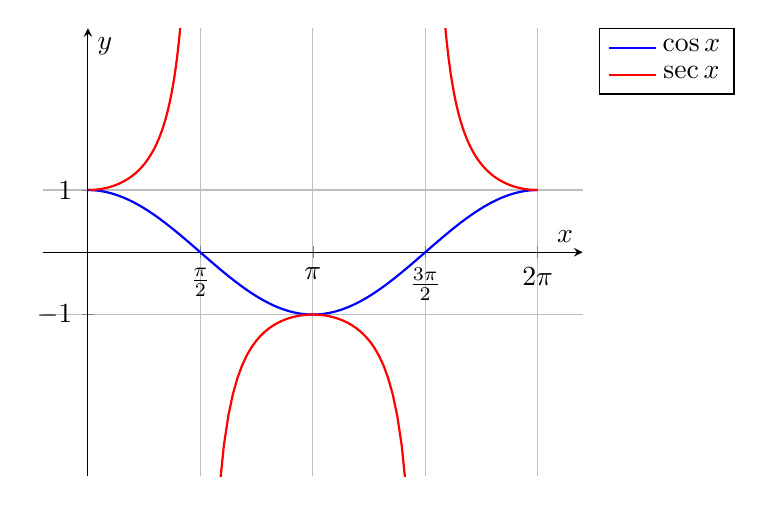
\begin{tikzpicture}
    \begin{axis}[
        domain=0:2*pi,
        samples=100,
        axis lines=middle,
        xlabel=$x$, ylabel=$y$,
        xtick={0, pi/2, pi, 3*pi/2, 2*pi},
        xticklabels={$0$, $\frac{\pi}{2}$, $\pi$, $\frac{3\pi}{2}$, $2\pi$},
        ytick={-1, 1},
        ymin=-3, ymax=3,
        grid=both,
        legend pos=outer north east,
        enlargelimits=true,
    ]
    \addplot [blue, thick] {cos(deg(x))};
    \addplot [red, thick, domain=0.01:pi/2-0.01, samples=50] {1/cos(deg(x))};
    \addplot [red, thick, domain=pi/2+0.01:3*pi/2-0.01, samples=50] {1/cos(deg(x))};
    \addplot [red, thick, domain=3*pi/2+0.01:2*pi-0.01, samples=50] {1/cos(deg(x))};
    \legend{$\cos x$, $\sec x$}
    \end{axis}
\end{tikzpicture}

Now, we will look at the key properties of the sine and cosecant functions.

\begin{tabular}{ |p{2cm}||p{5cm}|p{5cm}|  }
 \hline
 Property & $y = \sin x$ & $y = \csc x$\\
 \hline
 Period   & $2\pi$    & $2\pi$ \\
 \hline
 Max Value & 1 & N/A \textcolor{notecolor}{$\infty$ is NOT a value}\\
 \hline
 Min Value & -1 & N/A \textcolor{notecolor}{$\infty$ is NOT a value}\\
 \hline
 y-intercept & (0, 0) & N/A \\
 \hline
 x-intercept & 0, $\pi$, $2\pi$,... OR ($n\pi$, 0), $n\in \mathbb{Z}$(1)  & N/A\\
 \hline
 Vertical Asymptote & N/A & $x = n\pi, n\in \mathbb{Z}$ \textcolor{notecolor}{occurs at the x-int of $\sin x$}\\
 \hline
 Amplitude & 1 & N/A \textcolor{notecolor}{no max or min value}\\
 \hline
 Domain & $\{x\in \mathbb{R}\}$ & $\{x\in \mathbb{R}|x \neq n\pi, n\in \mathbb{Z} \}$\\
 \hline
 Range & $\{y\in \mathbb{R}|-1\leq y \leq 1\}$ & $\{y\in \mathbb{R}|y\leq -1, y \geq 1\}$\\
 \hline
\end{tabular}

\vspace{2em}

\textbf{Overview:} This unit consists of 5 video lessons. Allow no more than 12 class days for this unit, including time for review and to write the test.

\subsection{Graphs of Sine, Cosine and Tangent}
\[
\begin{array}{c}
y = \sin x \\
y = \cos x \\
y = \tan x \\
\end{array}
\]

\noindent Remember that \(\sin x\) is defined as the y-coordinate of the unit circle. This will be the distance above or below the x-axis.

\noindent For untransformed sinusoidal functions we have the following properties...

\subsubsection*{Example 1: Graph \( y = \sin x + 2 \)}
Vertical translation: now instead of oscillating around the x-axis, it will oscillate around the line \( y = 2 \).

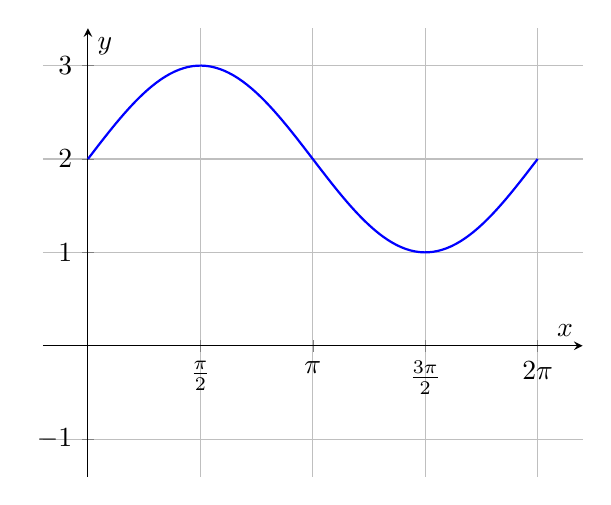
\begin{tikzpicture}
    \begin{axis}[
        domain=0:2*pi,
        samples=100,
        axis lines=middle,
        xlabel=$x$, ylabel=$y$,
        xtick={0, pi/2, pi, 3*pi/2, 2*pi},
        xticklabels={$0$, $\frac{\pi}{2}$, $\pi$, $\frac{3\pi}{2}$, $2\pi$},
        ytick={-1, 1, 2, 3},
        ymin=-1, ymax=3,
        grid=both,
        enlargelimits=true,
    ]
    \addplot [blue, thick] {sin(deg(x)) + 2};
    \end{axis}
\end{tikzpicture}

\subsubsection*{Example 2: Graph \( y = 2\cos x \) and \( y = -2\cos x \)}
Vertical stretch and reflection.

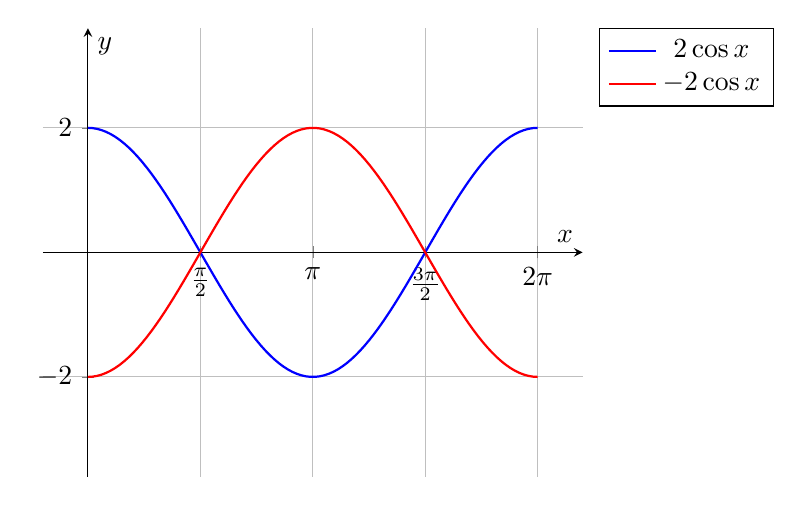
\begin{tikzpicture}
    \begin{axis}[
        domain=0:2*pi,
        samples=100,
        axis lines=middle,
        xlabel=$x$, ylabel=$y$,
        xtick={0, pi/2, pi, 3*pi/2, 2*pi},
        xticklabels={$0$, $\frac{\pi}{2}$, $\pi$, $\frac{3\pi}{2}$, $2\pi$},
        ytick={-2, 0, 2},
        ymin=-3, ymax=3,
        grid=both,
        legend pos=outer north east,
        enlargelimits=true,
    ]
    \addplot [blue, thick] {2*cos(deg(x))};
    \addplot [red, thick] {-2*cos(deg(x))};
    \legend{$2\cos x$, $-2\cos x$}
    \end{axis}
\end{tikzpicture}

\subsubsection*{Example 3: Graph \( y = \sin(x - \pi/2) \)}
Phase shift (horizontal translation) moves the function left or right.

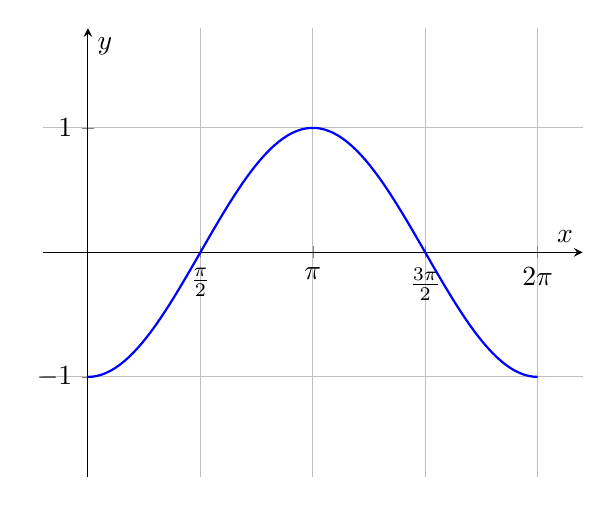
\begin{tikzpicture}
    \begin{axis}[
        domain=0:2*pi,
        samples=100,
        axis lines=middle,
        xlabel=$x$, ylabel=$y$,
        xtick={0, pi/2, pi, 3*pi/2, 2*pi},
        xticklabels={$0$, $\frac{\pi}{2}$, $\pi$, $\frac{3\pi}{2}$, $2\pi$},
        ytick={-1, 1},
        ymin=-1.5, ymax=1.5,
        grid=both,
        enlargelimits=true,
    ]
    \addplot [blue, thick] {sin(deg(x - pi/2))};
    \end{axis}
\end{tikzpicture}

\newpage

\subsection{Changing the Period}

\subsubsection*{Example 4: Graph the function \( y = \sin(3x) \)}
The 3 corresponds to a horizontal compression.

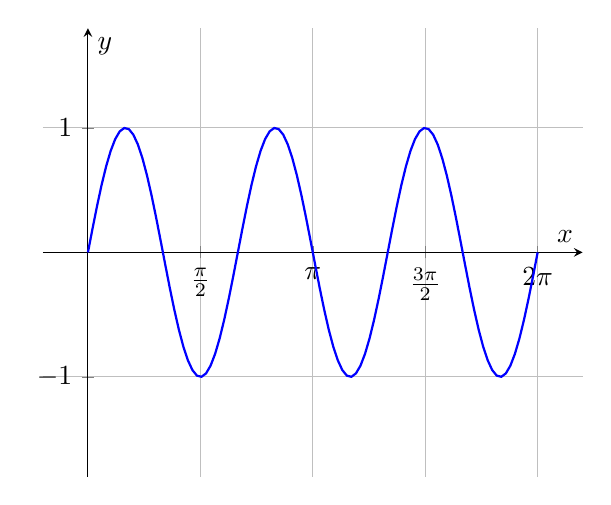
\begin{tikzpicture}
    \begin{axis}[
        domain=0:2*pi,
        samples=100,
        axis lines=middle,
        xlabel=$x$, ylabel=$y$,
        xtick={0, pi/2, pi, 3*pi/2, 2*pi},
        xticklabels={$0$, $\frac{\pi}{2}$, $\pi$, $\frac{3\pi}{2}$, $2\pi$},
        ytick={-1, 1},
        ymin=-1.5, ymax=1.5,
        grid=both,
        enlargelimits=true,
    ]
    \addplot [blue, thick] {sin(deg(3*x))};
    \end{axis}
\end{tikzpicture}

\subsubsection*{Example 5: Determine the value of \( k \) in \( y = \cos(kx) \) if the period is \( \pi/2 \)}

\[
\text{The period } T = \frac{2\pi}{k} = \frac{\pi}{2} \implies k = 4
\]

\newpage


\subsection{Reciprocal Trig Functions}
Complete the following graphs for \( y = \sec x \) and \( y = \cot x \).

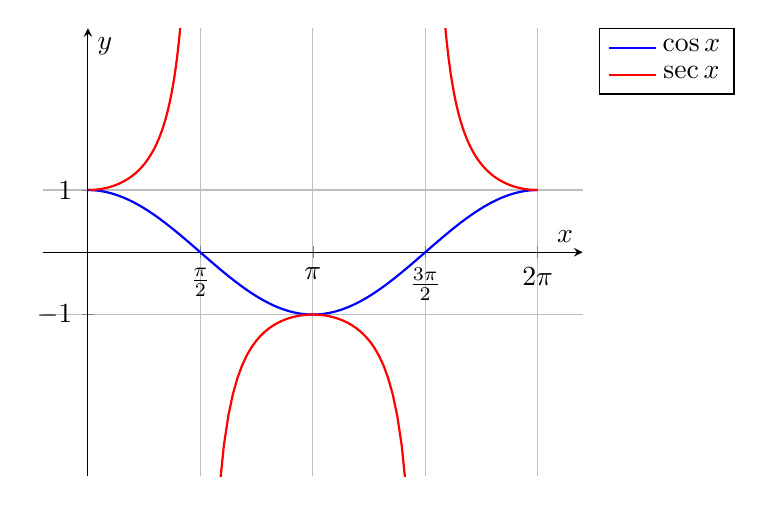
\begin{tikzpicture}
    \begin{axis}[
        domain=0:2*pi,
        samples=100,
        axis lines=middle,
        xlabel=$x$, ylabel=$y$,
        xtick={0, pi/2, pi, 3*pi/2, 2*pi},
        xticklabels={$0$, $\frac{\pi}{2}$, $\pi$, $\frac{3\pi}{2}$, $2\pi$},
        ytick={-1, 1},
        ymin=-3, ymax=3,
        grid=both,
        legend pos=outer north east,
        enlargelimits=true,
    ]
    \addplot [blue, thick] {cos(deg(x))};
    \addplot [red, thick, domain=0.01:pi/2-0.01, samples=50] {1/cos(deg(x))};
    \addplot [red, thick, domain=pi/2+0.01:3*pi/2-0.01, samples=50] {1/cos(deg(x))};
    \addplot [red, thick, domain=3*pi/2+0.01:2*pi-0.01, samples=50] {1/cos(deg(x))};
    \legend{$\cos x$, $\sec x$}
    \end{axis}
\end{tikzpicture}

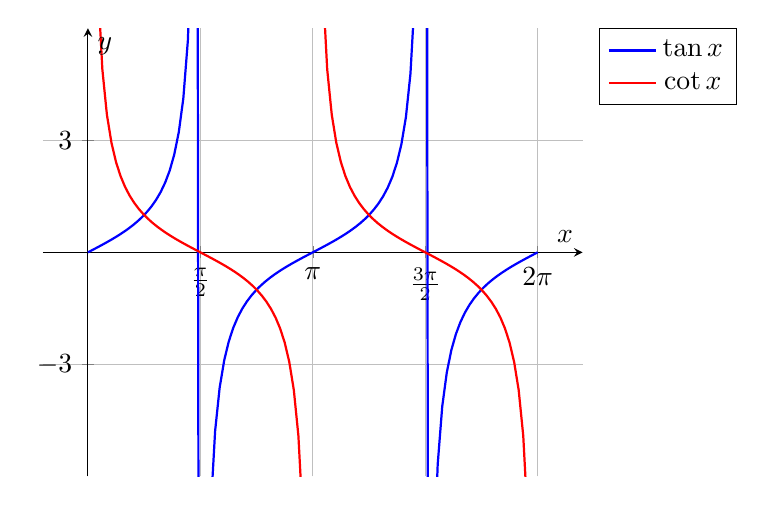
\begin{tikzpicture}
    \begin{axis}[
        domain=0:2*pi,
        samples=100,
        axis lines=middle,
        xlabel=$x$, ylabel=$y$,
        xtick={0, pi/2, pi, 3*pi/2, 2*pi},
        xticklabels={$0$, $\frac{\pi}{2}$, $\pi$, $\frac{3\pi}{2}$, $2\pi$},
        ytick={-3, 0, 3},
        ymin=-5, ymax=5,
        grid=both,
        legend pos=outer north east,
        enlargelimits=true,
    ]
    \addplot [blue, thick] {tan(deg(x))};
    \addplot [red, thick, domain=0.01:pi-0.01, samples=50] {1/tan(deg(x))};
    \addplot [red, thick, domain=pi+0.01:2*pi-0.01, samples=50] {1/tan(deg(x))};
    \legend{$\tan x$, $\cot x$}
    \end{axis}
\end{tikzpicture}

\newpage


\subsection{Sinusoidal Functions}
The general form of a sinusoidal function is:
\[
f(x) = a \sin [k (x - d)] + c
\]

\noindent Vertical Stretch: \( |a| > 1 \) \\
Vertical Compression: \( |a| < 1 \) \\
Reflection in x-axis: \( a < 0 \) \\
Horizontal Stretch: \( |k| < 1 \) \\
Horizontal Compression: \( |k| > 1 \) \\
Reflection in y-axis: \( k < 0 \) \\
Phase Shift: horizontal translation \\
Vertical translation: up \( c > 0 \), down \( c < 0 \)

\subsubsection*{Example 1: Graph \( y = 2\sin(\pi(x + 1)) - 3 \)}

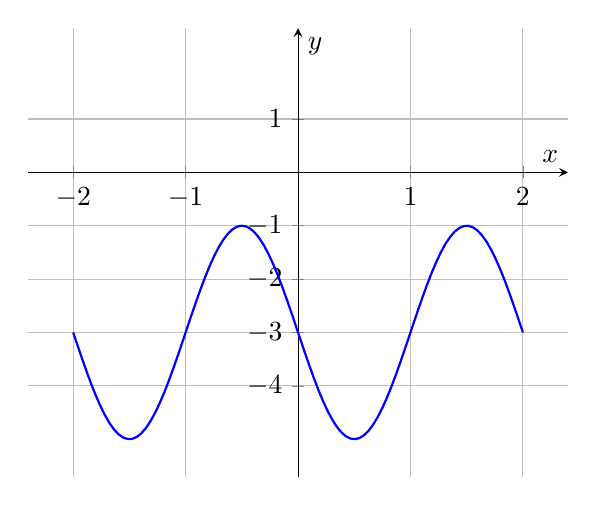
\begin{tikzpicture}
    \begin{axis}[
        domain=-2:2,
        samples=100,
        axis lines=middle,
        xlabel=$x$, ylabel=$y$,
        xtick={-2, -1, 0, 1, 2},
        ytick={-4, -3, -2, -1, 0, 1},
        ymin=-5, ymax=2,
        grid=both,
        enlargelimits=true,
    ]
    \addplot [blue, thick] {2*sin(deg(pi*(x + 1))) - 3};
    \end{axis}
\end{tikzpicture}

\subsubsection*{Example 2: Graph \( y = -5\cos(3x) + 1 \)}

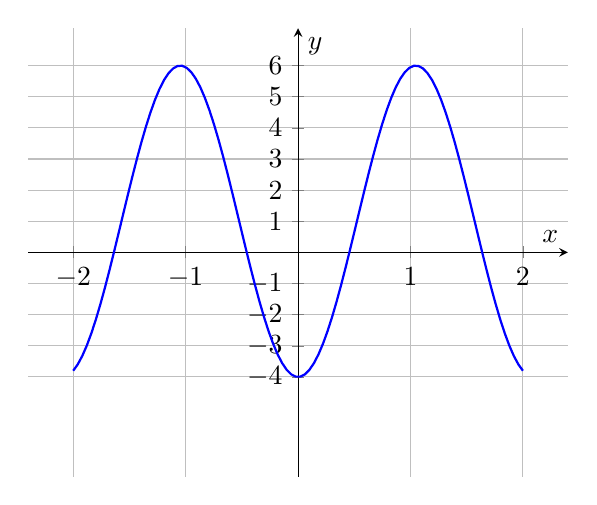
\begin{tikzpicture}
    \begin{axis}[
        domain=-2:2,
        samples=100,
        axis lines=middle,
        xlabel=$x$, ylabel=$y$,
        xtick={-2, -1, 0, 1, 2},
        ytick={-4, -3, -2, -1, 0, 1, 2, 3, 4, 5, 6},
        ymin=-6, ymax=6,
        grid=both,
        enlargelimits=true,
    ]
    \addplot [blue, thick] {-5*cos(deg(3*x)) + 1};
    \end{axis}
\end{tikzpicture}

\subsubsection*{Example 3: Find the form of the cosine curve that has an amplitude of 4, a period of \( 2\pi \), a left phase shift of \( \pi/4 \), and a vertical translation of 7.}

\[
y = 4\cos\left(x + \frac{\pi}{4}\right) + 7
\]

\subsubsection*{Example 4: Sketch the transformation of \( f(x) = \sin x \) with an amplitude of 3, period \( 2\pi \), and a phase shift of 0.5 radians to the right.}

\[
y = 3\sin\left(x - 0.5\right)
\]

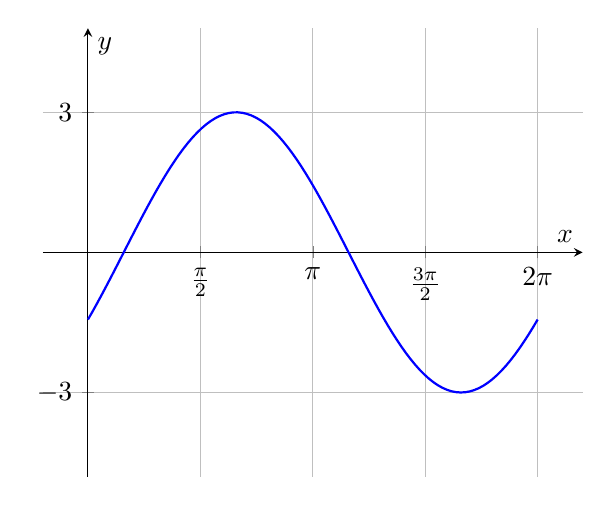
\begin{tikzpicture}
    \begin{axis}[
        domain=0:2*pi,
        samples=100,
        axis lines=middle,
        xlabel=$x$, ylabel=$y$,
        xtick={0, pi/2, pi, 3*pi/2, 2*pi},
        xticklabels={$0$, $\frac{\pi}{2}$, $\pi$, $\frac{3\pi}{2}$, $2\pi$},
        ytick={-3, 0, 3},
        ymin=-4, ymax=4,
        grid=both,
        enlargelimits=true,
    ]
    \addplot [blue, thick] {3*sin(deg(x - 0.5))};
    \end{axis}
\end{tikzpicture}

\newpage

\subsection{Solving Trigonometric Equations}

\subsubsection*{Example 1: Determine the solution to the equation \( 2\sin x + 1 = 0 \) for \( x \) in \([0, 2\pi]\)}

\[
2\sin x + 1 = 0 \implies \sin x = -\frac{1}{2}
\]
\[
x = \frac{7\pi}{6}, \frac{11\pi}{6}
\]

\subsubsection*{Example 2: Determine the solution to the equation \( 3(\tan x + 1) = 2 \) for \( x \) in \([0, 2\pi]\)}

\[
3(\tan x + 1) = 2 \implies \tan x = -\frac{1}{3}
\]
\[
x = \arctan\left(-\frac{1}{3}\right), \pi + \arctan\left(-\frac{1}{3}\right)
\]

\subsubsection*{Example 3: Determine the solution to the equation \( 2\sin^2 x - 3\sin x + 1 = 0 \) for \( x \) in \([0, 2\pi]\)}

\[
2\sin^2 x - 3\sin x + 1 = 0 \implies (2\sin x - 1)(\sin x - 1) = 0
\]
\[
\sin x = \frac{1}{2}, 1
\]
\[
x = \frac{\pi}{6}, \frac{5\pi}{6}, \frac{\pi}{2}
\]

\subsubsection*{Example 4: Determine the solution to the equation \( 2\sec^2 x - 3 + \tan x = 0 \) for \( x \) in \([0, 2\pi]\)}

\[
2\sec^2 x - 3 + \tan x = 0 \implies 2(1 + \tan^2 x) - 3 + \tan x = 0 \implies 2\tan^2 x + \tan x - 1 = 0
\]
\[
(2\tan x - 1)(\tan x + 1) = 0 \implies \tan x = \frac{1}{2}, -1
\]
\[
x = \arctan\left(\frac{1}{2}\right), \pi + \arctan\left(\frac{1}{2}\right), \arctan(-1), \pi + \arctan(-1)
\]

\subsubsection*{Example 5: Determine the solution to the equation \( 3\sin x + 3\cos^2 x = 2 \) for \( x \) in \([0, 2\pi]\)}

\[
3\sin x + 3\cos^2 x = 2 \implies 3\sin x + 3(1 - \sin^2 x) = 2 \implies 3\sin x + 3 - 3\sin^2 x = 2
\]
\[
-3\sin^2 x + 3\sin x + 1 = 0 \implies 3\sin^2 x - 3\sin x - 1 = 0
\]
\[
(3\sin x + 1)(\sin x - 1) = 0 \implies \sin x = -\frac{1}{3}, 1
\]
\[
x = \arctan(-\frac{1}{3}), \pi + \arctan(-\frac{1}{3}), \frac{\pi}{2}
\]

\newpage

\subsection{Making Connections to the "Real World"}

\subsection*{Making Connections}
We are going to use the graphing calculators for instantaneous rate of change.

\noindent On the graphing calculator:
\begin{itemize}
    \item Graph the curve \( y = \sin x \) (adjust your window so you see the curve better)
    \item Use the DRAW button \texttt{[2nd PRGM]} to draw on a tangent line
    \item Press \texttt{2nd PRGM}, choose 5: Tangent
    \item It will take you back to the graph, key in the x-value where you want the tangent line and press enter. Fill in the following table.
\end{itemize}

\noindent Many "real world" applications follow a cyclical or sinusoidal pattern. We can use a sinusoidal curve to model them. Usually we will choose the sine curve and apply a transformation to suit.

\subsubsection*{Example 1: The number of employees at a City Bicycle Company for each of the last 11 years is shown below. Find a sine curve that will model this data. Use technology to help you.}

\begin{minipage}{0.45\textwidth}
\begin{tabbing}
\hspace{1cm} \= \hspace{2cm} \= \kill
\textbf{Year} \hspace{1cm} \= \textbf{Employees} \\
1 \> 228 \\
2 \> 241 \\
3 \> 259 \\
4 \> 233 \\
5 \> 226 \\
6 \> 209 \\
7 \> 212 \\
8 \> 225 \\
9 \> 240 \\
10 \> 251 \\
11 \> 261 \\
\end{tabbing}
\end{minipage}

\begin{minipage}{0.45\textwidth}
\subsubsection*{Solution}
\begin{align*}
\text{Amplitude (half the distance from max to min):} & \\
261 - 209 &= 52 \\
\frac{52}{2} &= 26 \\
\\
\text{Midline (the horizontal line right between max and min):} & \\
\frac{261 + 209}{2} &= 235 \\
\\
\text{Period (for k-value):} & \\
11 - 3 &= 8 \\
P = \frac{2\pi}{k} \implies 8 &= \frac{2\pi}{k} \\
8k &= 2\pi \\
k &= \frac{2\pi}{8} \implies k = \frac{\pi}{4} \\
\\
\text{Phase Shift (the x-value when the y is first on the midline):} & \\
& 1.3 \\
\end{align*}
\end{minipage}

\noindent The equation of the sine curve modeling the data is:
\[
y = 26\sin\left(\frac{\pi}{4}(x - 1.3)\right) + 235
\]
\newpage


\section{Unit 6}
\subsection{Logarithms}

\begin{lessonbox}{Introduction to Logarithms}
As we saw last class, the logarithm function is the inverse of an exponential. But what exactly does this mean?

\[
\begin{aligned}
    &\text{If } f(x) = 2^x \text{ then } f^{-1}(x) = \log_2(x)\\
    &\text{The function returns the value of a power when given an exponent.}\\
    &\text{The logarithm returns the exponent when given the value of a power.}
\end{aligned}
\]
\end{lessonbox}

\begin{examplebox}{Example 1: Converting between Logarithmic and Exponential Forms}
Write the equivalent log or exponential equation.
\begin{align*}
    \text{a) } \log_2{16} = 4 &\quad \leftrightarrow \quad 2^4 = 16\\
    \text{b) } 7^2 = 49 &\quad \leftrightarrow \quad \log_7{49} = 2\\
    \text{c) } 5^x = 11 &\quad \leftrightarrow \quad \log_5{11} = x\\
    \text{d) } \log_x{42} = 7 &\quad \leftrightarrow \quad x^7 = 42
\end{align*}
\end{examplebox}

\begin{examplebox}{Example 2: Evaluating Logarithms}
Evaluate the following logs:
\begin{align*}
    \text{a) } \log_{10}{100} &= 2\\
    \text{b) } \log_2{64} &= 6\\
    \text{c) } \log_2{\left(\frac{1}{2}\right)} &= -1\\
    \text{d) } \log_3{\left(\frac{1}{27}\right)} &= -3
\end{align*}
\end{examplebox}

\begin{examplebox}{Example 3: Estimating Logarithms}
Estimate \(\log_3{10}\).

The calculator has two log buttons: \(\log\) and \(\ln\) (base 10 and base \(e \approx 2.7183\), respectively).
\end{examplebox}

\begin{examplebox}{Example 4: Using a Calculator to Evaluate Logarithms}
Use a calculator to evaluate, then write an equivalent exponential equation.
\begin{align*}
    \text{a) } \log{52} &\approx 1.716 \quad \leftrightarrow \quad 10^{1.716} = 52\\
    \text{b) } \log{24} &\approx 1.380 \quad \leftrightarrow \quad 10^{1.380} = 24\\
    \text{c) } \ln{12} &\approx 2.485 \quad \leftrightarrow \quad e^{2.485} = 12
\end{align*}
\end{examplebox}

\subsection{Power Law of Logarithms}

\begin{lessonbox}{Understanding the Power Law of Logarithms}
Evaluate each pair of logarithms on your calculator - What do you notice?
\begin{align*}
    \text{a) } 4 \log{2} &\quad \log{16}\\
    \text{b) } 2 \log{3} &\quad \log{9}\\
    \text{c) } 2 \log{5} &\quad \log{25}
\end{align*}

\textbf{Proof:} Let \( w = \log_b{x} \). Therefore, \( b^w = x \).

\textbf{What use is the power law?}
\begin{enumerate}
    \item It can help simplify logarithmic expressions.
    \item It gives us a method for solving exponential equations.
\end{enumerate}
\end{lessonbox}

\begin{examplebox}{Example 1: Evaluating Logarithms Using the Power Law}
Evaluate the following logarithms:
\begin{align*}
    \text{a) } \log_2{8} &= 3 \quad \text{(Change 8 to } 2^3)\\
    \text{b) } \log_3{\sqrt{27}} &= \frac{3}{2}
\end{align*}
\end{examplebox}

\begin{examplebox}{Example 2: Solving Exponential Equations Using Logarithms}
Solve by first taking the log of both sides and using the power law of logarithms:
\begin{align*}
    \text{a) } 5^t &= 15625 \quad \leftrightarrow \quad t \log{5} = \log{15625} \quad \leftrightarrow \quad t = \frac{\log{15625}}{\log{5}} = 6\\
    \text{b) } 1000 &= 2000(1+0.2)^n \quad \leftrightarrow \quad \frac{1000}{2000} = (1.2)^n \quad \leftrightarrow \quad n = \frac{\log{0.5}}{\log{1.2}} \approx -3.106
\end{align*}
\end{examplebox}

\begin{examplebox}{Example 3: Evaluating Logarithms Using the Change of Base Formula}
Evaluate \(\log_3{54}\):

First, let the expression equal a variable and turn it into the equivalent exponential expression. This actually gives us the change of base formula...
\[
\log_b{m} = \frac{\log{m}}{\log{b}}
\]
\end{examplebox}

\begin{examplebox}{Example 4: Using the Change of Base Formula}
Use the change of base formula to evaluate \(\log_8{254}\):
\[
\log_8{254} = \frac{\log{254}}{\log{8}} \approx 2.9
\]
\end{examplebox}

\begin{examplebox}{Example 5: Solving Compound Interest Problems Using Logarithms}
An investment of \$2000 earns 2\% interest, compounded yearly. A formula to represent this situation is:
\[
A = 2000 (1.02)^n
\]
where \( A \) is the amount of the investment and \( n \) is the number of years of the investment. How long before the investment doubles?
\[
2 = (1.02)^n \quad \leftrightarrow \quad n = \frac{\log{2}}{\log{1.02}} \approx 35
\]
\end{examplebox}

\subsection{Equivalent Exponential Expressions}

\begin{examplebox}{Example 1: Rewriting Exponentials Using a Different Base}
Rewrite the following using a base of 3.
\[
36 \quad \leftrightarrow \quad 3^6 = (3^2)^3 = 9^3
\]
\end{examplebox}

\begin{examplebox}{Example 2: Using Logarithms to Find the Value of an Exponent}
Use logarithms to find the value of an exponent: \( 3^x = 11 \)
\[
x = \frac{\log{11}}{\log{3}} \approx 2.183
\]
\end{examplebox}
\begin{examplebox}{Example 3: Solve for \( x \) by first writing as powers with the same base.}
\begin{align*}
    27^x &= 9^{2x-3} \implies (3^3)^x = (3^2)^{2x-3} \\ 
    3^{3x} &= 3^{4x-6}  \\
    3x &= 4x-6 x = 6
\end{align*}
\end{examplebox}
\subsection{Techniques for Solving Exponential Equations}
\begin{lessonbox}{Techniques for Solving Exponential Equations}


Last lesson we solved exponential equations by forcing them to have an equal base and equating their exponents. But what about a situation like this:
\[
5^{2x+4} = 3^{x-7}
\]
\end{lessonbox}

\noindent \textbf{Problem:} We can't simply write them with the same base.\\
\textbf{Solution:} If we take the log of both sides, we can get the variables out of the exponent!

\begin{examplebox}{Example 1: Solve for \( x \)}
\begin{align*}
    \log{5^{2x+4}} &= \log{3^{x-7}}\\
    (2x+4) \log{5} &= (x-7) \log{3}\\
    2x \log{5} + 4 \log{5} &= x \log{3} - 7 \log{3}\\
    2x \log{5} - x \log{3} &= -7 \log{3} - 4 \log{5}\\
    x (2 \log{5} - \log{3}) &= -7 \log{3} - 4 \log{5}\\
    x &= \frac{-7 \log{3} - 4 \log{5}}{2 \log{5} - \log{3}} \approx -4.54
\end{align*}
\end{examplebox}
\begin{examplebox}{Example 2: Solve for \( x \)}
\[
2^x - 2^{-x} = 4
\]
There's no immediate method to solve this, we have to make a couple of adjustments in order to solve. Notice it's somewhat similar to a quadratic equation in that the variables are in decreasing order. We are going to multiply through by \( 2^x \) and this will become more apparent.
\begin{align*}
    2^x (2^x) - 2^x (2^{-x}) &= 4 (2^x)\\
    2^{2x} - 1 &= 4 \cdot 2^x\\
    2^{2x} - 4 \cdot 2^x - 1 &= 0
\end{align*}
Let \( u = 2^x \):
\begin{align*}
    u^2 - 4u - 1 &= 0\\
    u = \frac{4 \pm \sqrt{16 + 4}}{2} = \frac{4 \pm \sqrt{20}}{2} = 2 \pm \sqrt{5}\\
    2^x &= 2 + \sqrt{5}\\
    x &= \log_2 (2 + \sqrt{5}) \approx 1.79
\end{align*}
\end{examplebox}

\begin{examplebox}{Example 3: Using a Half-Life}
An archaeological discovery of an unknown plant fossil has 1/8 the amount of radioactive carbon as plants have today. If the half-life of the carbon is 5730 years, how old is the fossil?
\[
A = A_0 \left(\frac{1}{2}\right)^{\frac{t}{h}}
\]
Given:
\begin{align*}
\frac{1}{8} = \left(\frac{1}{2}\right)^{\frac{t}{5730}} \\
2^3 = 2^{\frac{t}{5730}} \\
3 = \frac{t}{5730}\\
t = 3 \times 5730 = 17190 \text{ years}
\end{align*}

\end{examplebox}

\subsection{Log Laws}

\begin{lessonbox}{Log Laws}
Remember that there were laws for multiplying and dividing powers with the same base. We need to adapt these for use with logarithms.

\[
\log_b(m \cdot n) = \log_b{m} + \log_b{n}
\]
\[
\log_b\left(\frac{m}{n}\right) = \log_b{m} - \log_b{n}
\]
\end{lessonbox}

\begin{examplebox}{Example 1: Simplify using the laws of logarithms}
\begin{align*}
    \text{a) } \log{5} + \log{10} &= \log{(5 \cdot 10)} = \log{50}\\
    \text{b) } \log{12} - \log{2} &= \log{\left(\frac{12}{2}\right)} = \log{6}
\end{align*}
\end{examplebox}

\begin{examplebox}{Example 2: Simplify each expression}
\begin{align*}
    \text{a) } \log{(5a)} + \log{10} - \log{(2b)} &= \log{(5a \cdot 10)} - \log{(2b)} \\
    &= \log{\left(\frac{50a}{2b}\right)} = \log{\left(\frac{25a}{b}\right)}\\
    \text{b) } \log{x} + 6 \log{y} + 3 \log{z} &= \log{x} + \log{(y^6)} + \log{(z^3)} \\
    &= \log{(x \cdot y^6 \cdot z^3)}
\end{align*}
\end{examplebox}

\begin{examplebox}{Example 3: Evaluate}
\begin{align*}
    \text{a) } \log{50} + \log{10} - \log{5} &= \log{(50 \cdot 10)} - \log{5}\\
    &= \log{500} - \log{5} = \log{100} = 2\\
    \text{b) } 4 \log_{12}{2} + 2 \log_{12}{3}
    &= \log_{12}{(2^4)} + \log_{12}{(3^2)} \\
    &= \log_{12}{16} + \log_{12}{9} = \log_{12}{144}
\end{align*}
\end{examplebox}

\begin{examplebox}{Example 4: Simplify and state any restrictions}
\begin{align*}
    \text{a) } \log{(2x^2 + 9x - 5)} - \log{(x + 5)} &= \log{\left(\frac{2x^2 + 9x - 5}{x + 5}\right)}\\
    \text{b) } \log{(x+3)} + \log{(2x-5)} &= \log{((x+3)(2x-5))}
\end{align*}
\end{examplebox}

\subsection{Solving Log Equations}
\begin{lessonbox}{Solving Log Equations}
    
There are three main techniques involved in solving logarithmic equations:
\begin{enumerate}
    \item Use the definition of a logarithm to rewrite the equation as an exponential. Then solve using the techniques for exponential equations.
    \item First simplify using the laws of logarithms, and then rewrite as an exponential to solve.
    \item First simplify using the laws of logarithms and then equate the arguments of the logs on both sides of the equal sign.
\end{enumerate}
\end{lessonbox}

\begin{examplebox}{Example 1: Use the definition to change into an exponential. Solve for \( n \)}
\begin{align*}
\log_3{(n^2 - 3n + 5)} = 2 \\
3^2 = n^2 - 3n + 5 \\
9 = n^2 - 3n + 5 \\
0 = n^2 - 3n - 4 \\
(n-4)(n+1) = 0 \\
n = 4 \text{ or } n = -1
\end{align*}

\end{examplebox}

\begin{examplebox}{Example 2: Simplify and then apply the definition. Solve for \( p \)}
\begin{align*}
\log{(p+5)} - \log{(p+1)} = 3 \implies \log{\left(\frac{p+5}{p+1}\right)} = 3 \\
10^3 = \frac{p+5}{p+1} \\
1000 = \frac{p+5}{p+1}\\
1000(p+1) = p + 5 \\
1000p + 1000 = p + 5 \\
999p = -995\\
p = -\frac{995}{999} \approx -1
\end{align*}

\end{examplebox}

\begin{examplebox}{Example 3: Equating the arguments. Solve for \( x \)}
\begin{align*}
\log{(2x^2 - 7x - 4)} = \log{(2x + 16)} \\
2x^2 - 7x - 4 = 2x + 16 \\
2x^2 - 9x - 20 = 0 \\
(2x + 5)(x - 4) = 0 \\
x = -\frac{5}{2} \text{ or } x = 4
\end{align*}

\end{examplebox}

\subsection{More Equations}

\begin{examplebox}{Example 1: An exponential with a product in it}
\[
7(1.06^x) = 5.2 \quad \leftrightarrow \quad 1.06^x = \frac{5.2}{7} \quad \leftrightarrow \quad x = \frac{\log{\left(\frac{5.2}{7}\right)}}{\log{1.06}} \approx -5.68
\]
\end{examplebox}

\begin{examplebox}{Example 2: Logarithms where an answer doesn't work out}
\begin{align*}
\log_6{x} + \log_6{(x+1)} = 1 \implies \log_6{[x(x+1)]} = 1 
x(x+1) = 6^1 = 6 \\
x^2 + x - 6 = 0 \\
(x+3)(x-2) = 0 \\
x = -3 \text{ or } x = 2
\end{align*}


Note: \( x = -3 \) is not a valid solution as logarithms of negative numbers are undefined.
\end{examplebox}

\subsection{The Logarithmic Scale in Science}

\subsubsection{A. Earthquakes}
\begin{lessonbox}{The Logarithm Scale in the Physical Sciences}
The Richter Scale defines the magnitude of an earthquake as:
\[
M = \log{\left(\frac{I}{I_0}\right)}
\]
Where \( I \) is the earthquake intensity measured and \( I_0 \) is the intensity of a reference quake.
\end{lessonbox}

\begin{examplebox}{Example 1: Comparing Earthquake Magnitudes}
The California earthquake that interrupted the World Series in 1989 measured 6.9 on the Richter scale. The quake that caused the 2004 tsunami in Indonesia measured 9.2. How much more powerful was the Indonesian quake?

Intuitively:
The difference in magnitude is \( 9.2 - 6.9 = 2.3 \).

Using the Definition:
\[
10^{9.2} / 10^{6.9} = 10^{2.3} \approx 200
\]
The Indonesian earthquake was about 200 times more powerful.
\end{examplebox}

\subsubsection{B. Sound}
The decibel scale compares sound intensities:
\[
L = 10 \log{\left(\frac{I}{I_0}\right)}
\]
Where \( I \) is the intensity of the sound being measured and \( I_0 \) is the threshold of human hearing (the quietest sound we can hear).

\begin{examplebox}{Example 2: Decibel Calculation}
A sound is 5000 times more intense than one that is just audible. How many decibels is the sound?
\[
L = 10 \log{(5000)} \approx 10 \times 3.699 \approx 37
\]
\end{examplebox}

\begin{examplebox}{Example 3: Comparing Loudness}
A jet engine emits a 160 dB sound, while Niagara Falls is 90 dB. How many times louder than Niagara Falls is a jet engine?
\[
10^{160/10} / 10^{90/10} = 10^{16 - 9} = 10^7
\]
A jet engine is \( 10^7 \) times louder than Niagara Falls.
\end{examplebox}

\subsubsection{C. The pH Scale}
The acidity or alkalinity of a solution is given by the pH scale:
\[
\text{pH} = -\log{[H^+]}
\]
Where \([H^+]\) is the concentration of hydronium ions in the solution in mol/L.

\begin{examplebox}{Example 4: Calculating pH}
The hydronium ions in blood measure at a concentration of \( 4 \times 10^{-7} \) mol/L. What is the pH of blood?
\[
\text{pH} = -\log{(4 \times 10^{-7})} = -(\log{4} + \log{10^{-7}}) = -(\log{4} - 7) \approx -0.602 - 7 = 6.4
\]
\end{examplebox}

\begin{examplebox}{Example 5: Finding Hydronium Ion Concentration}
What is the concentration of hydronium ions in a pool if the pH is 8.2?
\[
8.2 = -\log{[H^+]} \quad \leftrightarrow \quad [H^+] = 10^{-8.2} \approx 6.3 \times 10^{-9} \text{ mol/L}
\]
\end{examplebox}
\end{document}